\documentclass[5p,times,authoryear]{elsarticle}

\usepackage{amsmath,amssymb}
\usepackage{booktabs}
\usepackage{array}
\usepackage{tabularx}
\usepackage{multirow}
\usepackage{makecell}
\usepackage{graphicx}
\usepackage{xcolor}
\usepackage{algorithm}
\usepackage{algpseudocode}
\algrenewcommand\algorithmicrequire{\textbf{Input}}
\algrenewcommand\algorithmicensure{\textbf{Output}}
\algrenewcommand\alglinenumber[1]{\footnotesize #1.}
\usepackage{tikz}
\usetikzlibrary{arrows.meta,positioning,shapes.geometric,calc,fit,backgrounds}
\usepackage{lineno}
\usepackage{microtype}
\usepackage[labelsep=period]{caption}
\setlength{\emergencystretch}{2.5em}
\usepackage[hidelinks]{hyperref}

\usepackage{amsthm}
\theoremstyle{plain}
\newtheorem{proposition}{Proposition}
\newtheorem{corollary}{Corollary}
\newcolumntype{L}[1]{>{\raggedright\arraybackslash}p{#1}}

% Notation
\newcommand{\sbar}{\bar{\sigma}_0}
\newcommand{\Vlow}{V^{*}_{\mathrm{low}}}
\newcommand{\Vhigh}{V^{*}_{\mathrm{high}}}
\newcommand{\Vzero}{V^{*}_{0}}
\newcommand{\Vlin}{V^{*}_{\mathrm{lin}}}
\newcommand{\VMEU}{V^{*}_{\alpha\text{-MEU}}}
\newcommand{\slow}{\sigma_{\mathrm{low}}}
\newcommand{\shigh}{\sigma_{\mathrm{high}}}
\newcommand{\blo}{\beta_{\mathrm{lo}}}
\newcommand{\bhi}{\beta_{\mathrm{hi}}}
\newcommand{\Db}{\Delta_{\beta}}
\newcommand{\aMEU}{\alpha\text{-MEU}}
\newcommand{\ER}{E_{\mathcal{R}}}
\newcommand{\eR}{e_{\mathcal{R}}}
\newcommand{\dedge}{d_{\mathrm{edge}}}
\newcommand{\dmember}{d_{\mathrm{member}}}
\newcommand{\PSDI}{\mathrm{PSDI}}
\newcommand{\SM}[1]{Supplementary Material #1}

\journal{Computers \& Industrial Engineering}
\keywordtitlesep{.\ }

\begin{document}
\linenumbers

\begin{frontmatter}

\title{Member-specific thresholds and contested-price intervals for stage-gate screening: A curvature-based real-options method under regulatory ambiguity}

\begin{abstract}
Stage-gate committees decide the timing of irreversible investments under regulatory ambiguity, and members weighting adverse evidence differently can reach different timing decisions at the same price. Real-options analysis reduces this decision to one project-level trigger, and committee decision support compresses member assessments into a score or ranking, so neither reports the price range over which member classifications differ. This study therefore derives one price threshold per member from affine combinations of the triggers at both ends of a volatility interval, so a committee can locate disagreement before any vote. The extreme thresholds bound a contested-price interval, and a unique critical weight splits members around the no-ambiguity anchor. Under the affine rule, curvature placed this weight above one half in standard-deviation units and below it in variance units. Against a pre-commitment $\alpha$-maxmin expected utility benchmark, the largest relative trigger error over the primary radii was 2.74\%. Small trigger errors did not guarantee identical classifications. Two fidelity criteria held only at radii up to 10\%, which caps affine-only release. Monte Carlo committee panels measured the investment-timing information lost by compressing member thresholds into one trigger. The member vector cut median price-axis loss by 88.5\% against the ex post best of four single-trigger summaries. In a carbon capture, utilization, and storage retrofit, all archived prices stayed below the lower edge in the reference case. In 15 of 32 sensitivity configurations, the highest archived price reached or exceeded this edge. The report thus shows before any vote whether the prevailing price is contested.
\end{abstract}

\begin{keyword}
Real options \sep Stage-gate screening \sep Regulatory ambiguity \sep Group decision support \sep CCUS investment
\end{keyword}

\end{frontmatter}

\section{Introduction}

Large, irreversible investments are commonly reviewed through a sequence of stage gates \citep{Cooper2008}. At each gate, a committee decides whether to commit to the project now or to defer it to a later review. When the decision concerns timing, real-options analysis reduces it to a single investment trigger \citep{McDonaldSiegel1986,DixitPindyck1994}. Commitment is warranted once project value reaches this trigger. A single trigger gives the review one compact criterion, which can be documented and recomputed at successive gates. When project cash flows are linked to an observable price, the screening boundary can be restated on the price axis. The committee then reads it in units it already monitors. In this paper, a trigger is a project-value quantity, and a threshold is its image on the price axis.

Committee members may receive the same engineering, cost, and policy evidence and still place different weights on adverse regulatory scenarios. An ambiguity-aware real-options analysis returns one project-level trigger under a representative ambiguity attitude, so member-level dispersion disappears at the modeling stage. Committee decision-support procedures can retain individual assessments, but they aggregate them into a score, a ranking, or a vote before reporting. In both cases, the assessments are compressed before their implied classifications are compared.

Member-level dispersion does not always change the classification at a gate. A price below every member threshold places all members in the wait region. A price at or above every threshold places all members in the invest region. A mixed classification arises only between the lowest and the highest member thresholds. The position of the price relative to the whole threshold set therefore determines whether one classification suffices. An aggregate score replaces this set with one number. The set can be recovered from the recorded calibration, ambiguity radius, and member weights. Changing these inputs can change the classification of the same prevailing price.

This paper determines when member heterogeneity changes the current gate classification. It reports this information without aggregating member thresholds in advance. All members share one ordered ambiguity set and differ only in their recorded weights on its adverse endpoint. Member triggers follow a closed-form affine endpoint rule. Its accuracy is measured against the $\alpha$-maxmin expected utility ($\aMEU$) optimum under the same model inputs. The two rules can classify the same price differently. The paper therefore also determines when the affine report can be released alone and when the benchmark must be recomputed.

The model represents one component of regulatory uncertainty as an ordered interval of forward volatilities around an anchor. The committee records one weight per member on the adverse endpoint of this interval, where the option to wait has the lowest value. Lower volatility reduces the value of waiting and lowers the trigger. The adverse endpoint is therefore the low-volatility endpoint.

The running example is a committee screening a carbon capture, utilization, and storage (CCUS) retrofit of a coal-fired power plant. The retrofit costs $1.585\times10^{9}$\,CNY and captures $1.69\times10^{6}$ tonnes of CO$_2$ per year \citep{Sun2024}. Project cash flows track an observable carbon price, so the member triggers become marginal carbon-price thresholds in Chinese Yuan per tonne (CNY/t). The smallest and largest thresholds bound the contested-price interval. The ambiguity radii of the gates come from a policy-text series. Its document identifiers and dates are recorded, so a reader with database access can retrieve the same documents.

The same construction determines whether each member trigger lies above or below the no-ambiguity anchor. The trigger is strictly increasing in volatility, so the two endpoint triggers differ. Exactly one weight in $[0,1]$, the critical weight, places a member trigger at the anchor. This weight splits the members into two groups around the anchor, and the split carries over to the price thresholds. One half is the weight at which the two endpoint triggers count equally.

The paper makes one main contribution and two supporting contributions. The main contribution is a member-indexed gate report. The report consists of the member-threshold vector and the contested-price interval bounded by its extremes. It yields a pre-vote test of whether the prevailing price receives the same classification under every member assessment. The two supporting contributions are analytical and methodological. The analytical contribution yields a location rule for the critical weight. Uniqueness follows from the strict monotonicity of the affine rule, and trigger curvature places the weight relative to one half. This curvature changes sign between the standard-deviation and variance coordinates. The direction of each member's shift is therefore a property of the declared coordinate. The methodological contribution yields a release rule for the report. Benchmark comparisons and a classification-fidelity analysis measure its accuracy in price units. In this analysis, small trigger errors could still change the invest-or-wait outcome. A finite-registry safeguard converts these accuracy limits into conditions for affine-only release, and each release can then be audited against the registered configurations.

The CCUS application produced two main results. First, unanimity depended on the configuration. Under the reference configuration, every archived price stayed below the contemporaneous lower interval edge. In 15 of the 32 sensitivity configurations, the highest archived price reached or exceeded this edge. Second, the common inputs moved the interval edges further than member disagreement did. A 10\% reduction in the cost-to-volume ratio $I/Q$ moved the lower edge by 11.34\,CNY/t. The widest interval under the reference profile along the reconstructed path was 6.63\,CNY/t.

The study therefore treats disagreement among committee members as a reported quantity with stated accuracy limits. Existing work on real options reports mostly project-level objects, and committee decision support reports mostly aggregated scores or rankings. The reporting gap addressed here lies between these two literatures.

\begin{table*}[!t]
\centering
\footnotesize
\renewcommand{\arraystretch}{1.05}
\textbf{Nomenclature}\\[2pt]
\begin{tabular}{@{}L{0.2\textwidth}L{0.77\textwidth}@{}}
\toprule
\multicolumn{2}{@{}l}{\textbf{Decision and valuation variables}}\\
$I$ & Investment (retrofit) cost\\
$V^{*}$ & Investment trigger value\\
$\Vlow$, $\Vhigh$ & Trigger at the lower and upper endpoints of the ambiguity set $\Sigma_t$\\
$\Vlin$, $\VMEU$ & Member trigger under the affine rule and under the pre-commitment benchmark, at the same recorded weight\\
$\Vzero$ & Trigger at the volatility anchor $\sbar$\\
$V_0$ & Pre-commitment benchmark reference value\\
$V^{*}(\alpha,t)$ & Member-specific trigger under the affine rule, Eq.~(\ref{eq:affine})\\
$P^{*}$ & Marginal carbon-price threshold, Eq.~(\ref{eq:price})\\
$P^{*}_{i}$ & Marginal carbon-price threshold of member $i$, equal to $P^{*}$ evaluated at $\alpha_i$\\
$P^{*}_{i,\mathrm{lin}}$ & Marginal carbon-price threshold of member $i$ under the affine rule, used by the safeguard distances\\
$P^{*}_{0}$ & No-ambiguity marginal carbon-price threshold, called the anchor threshold\\
$P_t$ & Prevailing effective carbon price at gate $t$\\
$C_t$ & Contested-price interval, $[\min_i P^{*}_i,\max_i P^{*}_i)$. When all member thresholds coincide, this half-open interval is empty and $B_t=0$\\
$B_t$ & Width of the contested-price interval, Eq.~(\ref{eq:interval})\\
$\tau$ & First hitting time of a candidate trigger in the benchmark problem\\
$V_{\tau}$ & Project value at the first hitting time $\tau$\\
$J^{\alpha}$ & Pre-commitment $\aMEU$ benchmark objective, Eq.~(\ref{eq:Jalpha})\\
$c$, $s$, $\Delta$ & Common per-tonne accounting adjustments, with $\Delta=c-s$\\
$L_{\mathrm{lin}}$, $U_{\mathrm{lin}}$ & Lower and upper edges of the affine contested-price interval $C_t$\\[2pt]
\multicolumn{2}{@{}l}{\textbf{Stochastic process and economic parameters}}\\
$\sbar$ & Positive forward-volatility anchor, $\sbar>0$, estimated from history in the application\\
$\sigma_p$ & Carbon-price volatility, forward parameter of the GBM process\\
$\slow$, $\shigh$ & Lower and upper volatility endpoints of $\Sigma_t$\\
$\mu_c$ & Annual carbon-price growth scenario, declared as a decision input\\
$r$ & Discount rate\\
$\delta$ & Net discount margin, $\delta=r-\mu_c$\\
$Q$ & Annual captured emissions (t/yr), net of the capture rate\\
$\blo$, $\bhi$ & Positive roots of the characteristic equation at the low-volatility and high-volatility endpoints of the declared ambiguity set\\
$\beta_1$ & Positive root of the characteristic equation, Eq.~(\ref{eq:char}), as a function of $\sigma_p$\\
$\beta_0$ & Shorthand for $\beta_1(\sbar)$, the root at the volatility anchor\\
$\Db$ & Spread between the roots at the two volatility endpoints, $\Db:=\blo-\bhi\ge 0$, strictly positive at a positive radius (Proposition~\ref{prop:benchmark})\\
$D_0$, $E_0$ & Auxiliary curvature terms in the closed-form $\tilde{\kappa}$, Eq.~(\ref{eq:kappa})\\[2pt]
\multicolumn{2}{@{}l}{\textbf{Ambiguity-radius and recorded-weight parameters}}\\
$\alpha$ & Recorded weight on the adverse endpoint under the $\alpha$-maxmin parameterization. It is elicited or configured before the gate and serves as a reporting input. At $\alpha=1$, the benchmark objective reduces to MEU\\
$\Sigma_t$ & Volatility ambiguity set, Eq.~(\ref{eq:ambset})\\
$h_t$ & Admissible ambiguity radius at gate $t$; in the application, $h_t=\min\{c_w w_t,(1-\epsilon)\sbar\}$\\
$c_w$ & Signal-to-radius scaling constant in the pre-cap map $h_t=c_w w_t$, $c_w\ge 0$\\
$\epsilon$ & Admissibility margin for the ambiguity-radius cap, $0<\epsilon<1$\\
$\rho$ & Relative ambiguity radius, $h/\sbar$. Marked variants denote other quantities, namely $\hat{\rho}_k$ (sample autocorrelation), Spearman $\rho$ (rank correlation), and $\rho_{\mathrm{retest}}$ (reliability)\\
$\tilde{\alpha}(h)$ & Critical weight at which the member trigger crosses the anchor trigger, for $h>0$, Eq.~(\ref{eq:critical}); $\tilde{\alpha}(0):=1/2$ by continuous extension\\
$\tilde{\alpha}_{\mathrm{lin}}$, $\tilde{\alpha}_{\mathrm{rec}}$, $\tilde{\alpha}_{\alpha\text{-MEU}}$ & Critical weight under the affine rule, the recursive rule, and the pre-commitment benchmark\\
$\sigma_{\mathrm{eff}}(\alpha)$ & Effective volatility of the recursive rule, $\sqrt{\alpha\slow^{2}+(1-\alpha)\shigh^{2}}$\\
$\alpha_{\min}$, $\alpha_{\max}$ & Smallest and largest recorded weights on a panel, which set the two interval edges\\
$\tilde{\kappa}(\sbar)$ & Volatility-channel curvature ratio, $V^{*\prime\prime}/(4V^{*\prime})$, Eq.~(\ref{eq:kappa})\\[2pt]
\multicolumn{2}{@{}l}{\textbf{Approximation and safeguard quantities}}\\
$\theta$ & Registered economic-calibration tuple $(r,\mu_c,\sbar)$\\
$\eR(\theta,\rho)$ & Registered refined-grid maximum of the normalized error between affine and benchmark member triggers, Eq.~(\ref{eq:safeguard})\\
$\ER(\theta,\rho)$ & Price-unit release envelope specific to a calibration and a radius, Eq.~(\ref{eq:safeguard})\\
$\dedge$, $\dmember$ & Price-edge and nearest-member distances used by the safeguard, Eq.~(\ref{eq:safeguard})\\
$\varepsilon_{\mathrm{num}}$ & Numerical tolerance added to the registered maximum error\\[2pt]
\multicolumn{2}{@{}l}{\textbf{Policy-text input quantities}}\\
$w_t$ & Quarterly rolling variability signal, the four-quarter population standard deviation of PSDI, Eq.~(\ref{eq:wt})\\
$\PSDI_t$ & Policy-semantic-dispersion index, Eq.~(\ref{eq:psdi})\\
$\bar{c}_t$ & Centroid of normalized document embeddings in period $t$\\[2pt]
\multicolumn{2}{@{}l}{\textbf{Abbreviations}}\\
$\aMEU$ & Alpha-maxmin expected utility\\
PSDI & Policy-semantic-dispersion index\\
\bottomrule
\end{tabular}
\par\smallskip
\parbox{0.97\textwidth}{\emph{Notes.} Symbols appearing in at least one numbered equation or at least six times in the mathematics are listed.}
\end{table*}


\section{Literature review}

A gate report built from member thresholds and a price-axis interval relates to three research streams. Ambiguity-aware real options provide the trigger analysis. Committee decision support provides the reporting context, and text-based uncertainty measures provide one application input. Each stream returns a different object to a review gate, and each leaves one gap for member-level screening.

\subsection{Real-options analytics for irreversible investment}

\citet{McDonaldSiegel1986} demonstrated the positive value of waiting under irreversibility and uncertainty. \citet{DixitPindyck1994} developed this result into the trigger analysis used here. \citet{NadarajahSecomandi2023} surveyed the uptake of this framework in the operations literature on energy assets. In this literature, the valuation target is an operational asset, and the flexibility is managerial. The retrofit examined here is such an asset, and the quantity of interest is the date of commitment. In the standard perpetual geometric Brownian motion (GBM) model, higher volatility raises the value of waiting and increases the investment trigger. When volatility is ambiguous in the sense of \citet{Ellsberg1961}, more than one law for the price process remains admissible. The trigger then depends on how this ambiguity is represented and evaluated.

\citet{NishimuraOzaki2007} placed Knightian ambiguity on the drift of the price process in an irreversible investment problem. They evaluated it under the maxmin expected utility (MEU) preferences of \citet{GilboaSchmeidler1989}. In their model, the worst-case prior reduces the value of waiting and accelerates commitment. \citet{TrojanowskaKort2010} extended the drift-ambiguity analysis to a finite project life. In their results, acceleration held only in the short run. The $\alpha$-maxmin generalization \citep{Ghirardato2004} assigns weight $\alpha$ to the worst-case prior and $1-\alpha$ to the best-case prior. It nests MEU at $\alpha=1$. Under this broader formulation, \citet{Schroder2011} showed the dependence of the decision on the ambiguity attitude as well as on the ambiguity. The subjective project value can rise, and commitment can become more attractive. Two decision makers facing the same objective situation may therefore act differently. \citet{Schroder2020} noted a further issue. Ambiguity models of this class, including $\aMEU$, are generally not dynamically consistent. A recursive solution of an optimal-stopping problem requires dynamic consistency. The direction of the effect of ambiguity on exercise timing also varies with the setting. In \citet{MiaoWang2011}, ambiguity could accelerate or delay option exercise. The direction depended on whether ambiguity affected continuation payoffs, termination payoffs, or both. These results do not transfer directly to volatility ambiguity. Drift and volatility enter the characteristic equation through different terms, so the comparative statics for drift ambiguity require rederivation. The benchmark in this paper is therefore a pre-commitment rule. It is compared with a recursive alternative, which is time-consistent by construction.

Several formulations also place ambiguity on volatility, and they address other decision questions. They can be sorted by the object each one returns. Four objects recur, and one formulation may return more than one of them. Formulations concerned with the worth of a claim return a value. The uncertain-volatility model of \citet{Avellaneda1995} bounds the price of a claim by evaluating it at the extremes of a volatility band. The $G$-expectation calculus of \citet{Peng2019} gives this band a coherent dynamic form, and \citet{EpsteinJi2013} carried the construction into asset pricing. Formulations concerned with how an agent should act return a policy. \citet{Matoussi2015} solved robust utility maximization in nondominated models through second-order backward stochastic differential equations. \citet{Kallblad2018} obtained dynamically consistent investment criteria under model uncertainty through robust forward preferences. Formulations concerned with stopping return a stopping region. Multiple-prior and time-consistent stopping treatments return this region or an equilibrium policy \citep{Riedel2009,HuangYu2021}. Formulations concerned with commitment return a single robust decision. Recursive multiple priors belong to this group \citep{ChenEpstein2002,EpsteinSchneider2003}. So do robust control \citep{HansenSargent2001} and distributionally robust optimization \citep{MohajerinKuhn2018}. They evaluate uncertainty at the level of the decision problem and return one decision robust over the whole set. A robust recursion returns the same type of object. A rectangularity condition preserves the structure of the Bellman recursion \citep{Iyengar2005}. The ambiguity set may also be a confidence region estimated from observed data \citep{Wiesemann2013}. The reported output remains one worst-case policy. \citet{MazzonTankov2024} worked under smooth ambiguity \citep{Klibanoff2005}. They reduced a coal-plant divestment problem with learning to a family of standard stopping problems. Their output is still the policy of a single decision maker. Values, policies, regions, and robust decisions are all indexed by the problem. None of the reviewed formulations returns the price range over which members disagree.

One strand of the ambiguity literature works with sets of valuations. In the Knightian decision theory of \citet{Bewley2002}, incomplete preferences represent ambiguity. One act ranks above another only if its expected utility is higher under every prior in the set. Some pairs remain unranked. An inertia assumption resolves them in favor of the status quo. An alternative is then adopted only when it dominates the status quo unanimously. \citet{RigottiShannon2005} carried this structure into general equilibrium, where incomplete preferences induce a set of valuations. The unanimity principle of \citet{Bewley2002} suggests an analogous reporting logic for stage-gate screening, because deferral is the incumbent option at a gate. A unanimous invest classification here records agreement among the recorded member rules at the prevailing price. Where unanimity fails, aggregation is one possible downstream step. Axiomatic treatments of this step exist for heterogeneous beliefs and ambiguity attitudes. \citet{Gilboa2004} restricted the Pareto principle to choices under identical beliefs. \citet{Cres2011} aggregated maxmin experts sharing a utility function. \citet{Danan2016} applied the Pareto criterion only to comparisons robust to belief imprecision. Each of these studies characterized a social criterion. The member-threshold vector precedes the aggregation step, and any aggregation is a declared downstream procedure.

The present method reports a vector of member triggers indexed by recorded weights before the collective choice. The contested-price interval is computed from this vector. A project-level formulation can supply such a vector only after an explicit member-indexing step. For the pre-commitment objective, this step solves the same scalar problem at each recorded weight. A time-consistent formulation yields scalar thresholds only under one condition. The equilibrium stopping region of every member must have a unique boundary in the same ordered state variable. The volatility set used here meets this condition.

The applied literature on CCUS retrofit timing also works at the project level. \citet{Compernolle2017} evaluated offshore enhanced oil recovery with CO$_2$ storage. \citet{Fan2023} and \citet{Li2026} examined the retrofit timing of coal-fired plants, and \citet{Sun2024} examined incentive design. \citet{Colombe2024} worked at the system level and derived a deployment plan through two-stage stochastic programming. These studies produced project-level or system-level decisions.

One line of theory indexes the option by the individual. \citet{Garlappi2017,Garlappi2022} examined group real options in which members hold heterogeneous beliefs and decide by voting. In their model, a representative median member cannot reproduce group behavior. Their analysis concerns group behavior after a vote, and the present report precedes any vote. The present setting differs from this literature in three respects. Heterogeneity enters through ambiguity attitudes, all members share the same information set, and ambiguity falls on volatility. \citet{Cardenas2025} extended this line to the timing of group investment decisions. In this model, members hold heterogeneous beliefs, and the rule of each member has a double continuation region. Disagreement can produce inertia and underinvestment even when every member would invest individually. The two boundaries delimit the continuation region of one member. The interval reported here measures the spread of one-sided thresholds across members, and the gate reports this spread without resolving it. \citet{Deeney2021} built a real-options decision support tool for research and development investment in CO$_2$ recycling. Their compound option structure carries technical and market risk and values the project. Across this stream, the reported object is a project-level trigger, a value, or a policy. Other formulations return a stopping region, a robust decision, or group behavior after a vote. In the reviewed work, member-level rules appear inside group models of voting or joint timing \citep{Garlappi2017,Cardenas2025}. The first gap is therefore the absence of a gate-level vector of one-sided member thresholds indexed by ambiguity attitude. This gap includes the position of such thresholds relative to the no-ambiguity anchor under volatility ambiguity.

\subsection{Stage-gate screening and committee-level decision support}

Stage-gate processes organize investment evaluation as sequential committee reviews \citep{Cooper2008}. The supporting decision systems typically deliver aggregate scores, rankings, or recommendations \citep{Sprague1980,Power2002}. These outputs are updated as conditions change \citep{Violos2025}. Group decision methods such as TOPSIS-based scoring \citep{HwangYoon1981} also compress heterogeneous evaluations into a single score or ranking. A score ranks alternatives at one decision point. A member-specific threshold is the level of the state variable at which the screening classification of a member changes. A committee can use both. The thresholds locate the prevailing price relative to each member, and a scoring procedure ranks the remaining alternatives. The interval width measures dispersion among model-implied screening thresholds in price units. Consensus measures, reviewed by \citet{HerreraViedma2014}, assess alignment among stated preferences before a collective choice.

A separate operational-research tradition treats disagreement as an output of the analysis. \citet{Phillips1984} built the decision model jointly with the problem owners. The model counted as requisite once further sensitivity analysis generated no new intuitions. \citet{FrancoMontibeller2010} developed this stance into facilitated modeling for groups. The present method offers a quantitative device for this tradition in one setting. It quantifies the threshold implications of recorded weights without a further aggregation step. Aggregation procedures, and procedures deciding above the individual member, both operate downstream of this report. \citet{Dong2026} integrated information across attributes and periods to produce superiority-probability comparisons and probabilistic rankings. \citet{SongLi2026} represented numerical and linguistic preference relations and aggregated them at the subgroup level. They then solved minimum-adjustment consensus models under limited compromise. Portfolio and multi-stage models kept the decision above the individual member \citep{Marques2022,ShenLi2023,Saiz2024}. Recent robust and adaptive designs did so as well \citep{Shen2025,ShavazipourStewart2026}. Robust and adaptive designs use an uncertainty set to select one policy with acceptable performance across the set. These studies address what the organization should commit to. The present method examines whether the individuals screening one project currently agree, and by how much in carbon-price units. For each member, it reports the signed margin, defined as the member threshold minus the prevailing price. The margin is positive under a wait classification. At the committee level, the method reports the interval edges. Aggregating the edges away at the gate would leave a single number without a record of the member behind it. A consensus model, a ranking, or a portfolio selection could use them at a later stage. It would need a stated rule for how member thresholds enter its objectives and constraints. Most reviewed methods aggregate or reconcile member assessments before reporting, and facilitated modeling lacks a quantitative threshold device. No reviewed method converts recorded member weights into thresholds on the price axis, and this missing report is the second gap.

Recording these weights requires an elicitation step. An elicitation instrument must meet three requirements. It must return a number in $[0,1]$ on the adverse endpoint of the declared ambiguity set. A calibration to a different object needs a stated mapping. It must be reproducible at the same gate, because the recorded weight determines the member threshold and enters the gate audit record. Its precision must be assessed against the review band around the critical weight, and a member inside this band receives a de-emphasized label. Matching-probability tasks, lottery equivalents, and structured vignettes meet the first requirement under a stated mapping. The second and third requirements constrain administration. They translate into a precision target for testing a candidate protocol before any gate.

\subsection{Text-based uncertainty measures as a model input}

In the application, only one gate input, the ambiguity radius, comes from policy text.

Existing studies commonly derive text-based uncertainty measures from keyword frequencies or supervised classifiers. The Economic Policy Uncertainty index counts prespecified newspaper terms \citep{Baker2016}. Investment research often uses it as a regression covariate \citep{GulenIon2016}. \citet{Hassan2019} extended this design to firm-level political risk, and \citet{Gavriilidis2021} applied it to climate news. Fixed term lists may miss paraphrases and emerging terminology. \citet{Hartley2025} reported closer agreement with human-audited labels for large language model classifiers than for dictionary rules. Whether policy documents carry a usable dispersion signal remained open in this comparison. Supervised alternatives include the MacBERT-based climate policy uncertainty index for China of \citet{Ma2023}. Such classifiers require labeled training data. The limits of fixed term lists and labeled data motivate the unsupervised, embedding-based construction in the application. The construction follows the text-as-data approach reviewed by \citet{Gentzkow2019}. The resulting series measures semantic dispersion across contemporaneous policy documents. In the reviewed studies, text-based measures served as indices, document labels, or regression covariates. None of them supplied an input to a member-level screening rule, which is the third gap.

Table~\ref{tab:lit} summarizes the three gaps. First, the reviewed real-options formulations return project-level objects or group behavior, and none reports a gate-level vector of member thresholds indexed by ambiguity attitude. Second, committee decision support aggregates member assessments into scores, rankings, or consensus measures, so the price range of member disagreement stays unreported. Third, text-based uncertainty measures have not been linked to member-level screening rules. The present method addresses the first two gaps with a member-indexed threshold vector on the price axis. A critical weight locates this vector relative to the anchor, and a stated accuracy standard sets its release conditions. For the third gap, the application supplies a replaceable text-based radius as one gate input. Such a vector depends on a precise statement of the gate decision and of the inputs shared by all members.

\begin{table*}[!t]
\caption{Relation of prior literature streams to the contested-price interval and its width. The first two rows are the streams underlying the method. The third row is the application-specific input of the running example.}
\label{tab:lit}
\centering
\footnotesize
\renewcommand{\arraystretch}{1.15}
\begin{tabular}{@{}L{0.27\textwidth}L{0.18\textwidth}L{0.22\textwidth}L{0.25\textwidth}@{}}
\toprule
Literature stream & Contribution & Gap for stage-gate screening & Role in this paper\\
\midrule
Ambiguity-aware real options \citep{NishimuraOzaki2007,TrojanowskaKort2010,Schroder2011,Fan2023} & Investment timing rules under non-unique priors & Member-level decomposition of the trigger at a review gate & Analytical basis for member triggers\\
Decision support and stage-gate screening \citep{Sprague1980,Cooper2008,ShenLi2023,Saiz2024,Shen2025,Violos2025} & Structured review processes and governance outputs & Explicit reporting of member-threshold dispersion from recorded weights & Interface logic reporting the contested-price interval, its width, and the current classification summary\\
Application input. Text-based policy-uncertainty measurement \citep{Baker2016,Gavriilidis2021,Ma2023,Hartley2025} & Quantitative signals from policy and news text & Integration of such signals into member-specific gate-level screening rules & Construction of the replaceable input $w_t$\\
\bottomrule
\end{tabular}
\end{table*}

\section{Decision setting and model inputs}

The gate decision and its inputs come first, because every reported threshold depends on them. Some inputs are shared by all members, and one input varies across members.

\subsection{The gate-level decision problem}

Consider a sequence of review gates. At each gate, a project receives a binary invest-or-wait classification before the committee makes its collective decision. The committee also specifies an interval of forward volatilities, called the ambiguity set of the gate. Eq.~(\ref{eq:ambset}) parameterizes this set by a single radius around an anchor. Members share a common regulatory information set. Heterogeneity enters only through the weight $\alpha_i\in[0,1]$ recorded for member $i$ on the adverse endpoint of the ambiguity set.

The method takes a calibration $\theta=(r,\mu_c,\sbar)$ and the project inputs $I$ and $Q$. It also takes the declared ambiguity radius $h_t$, the recorded weights $\{\alpha_i\}_{i=1}^{m}$, and the prevailing price $P_t$. It returns the member-specific price thresholds and a classification of $P_t$ as unanimous wait, mixed, or unanimous invest. It also states whether the affine report may be released alone or requires a benchmark recomputation.

Figure~\ref{fig:architecture} organizes these inputs and outputs into three layers. The input layer supplies the radius and the prevailing price. The analytical layer produces the member triggers and the critical weight. The interface layer converts the triggers into price-axis thresholds and applies the release rule. It then issues either an affine-only report or a dual report containing both the affine and the benchmark results.

\begin{figure*}[!t]
\centering
\resizebox{0.97\textwidth}{!}{%
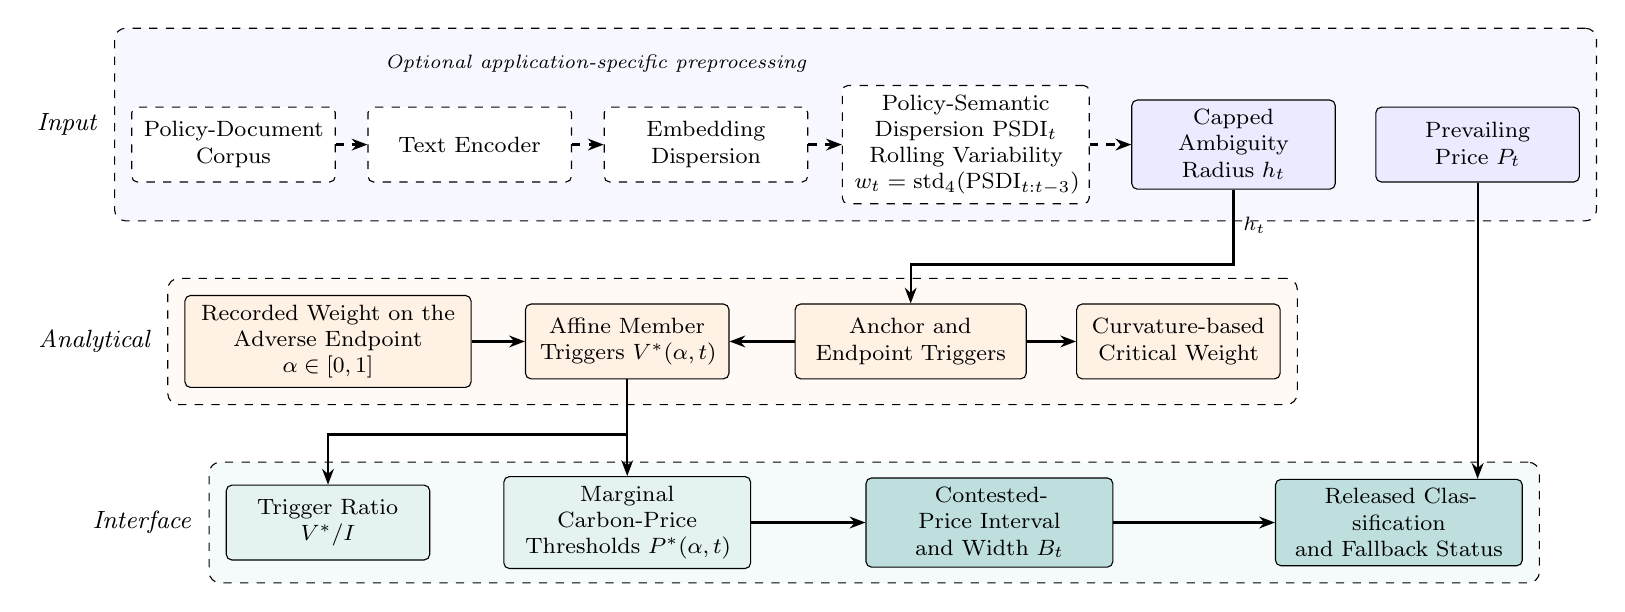
\begin{tikzpicture}[
  font=\footnotesize,
  box/.style={draw, rounded corners=2pt, align=center, minimum height=0.95cm, text width=2.35cm, fill=white},
  dbox/.style={box, dashed},
  arr/.style={-{Stealth[length=2mm]}, thick},
  darr/.style={-{Stealth[length=2mm]}, thick, dashed},
  layer/.style={draw, dashed, rounded corners=4pt, inner sep=6pt}
]
% Input layer
\node[dbox] (corpus) at (0,0) {Policy-Document\\Corpus};
\node[dbox] (enc) at (3.0,0) {Text Encoder};
\node[dbox] (emb) at (6.0,0) {Embedding\\Dispersion};
\node[dbox, text width=2.9cm, minimum height=1.25cm] (psdi) at (9.3,0) {Policy-Semantic Dispersion $\PSDI_t$\\Rolling Variability\\$w_t=\mathrm{std}_4(\PSDI_{t:t-3})$};
\node[box, fill=blue!8] (radius) at (12.7,0) {Capped Ambiguity\\Radius $h_t$};
\node[box, fill=blue!8] (price) at (15.8,0) {Prevailing\\Price $P_t$};
\draw[darr] (corpus) -- (enc);
\draw[darr] (enc) -- (emb);
\draw[darr] (emb) -- (psdi);
\draw[darr] (psdi) -- (radius);
\node[font=\scriptsize\itshape, anchor=south] (optlab) at (4.6,0.8) {Optional application-specific preprocessing};
% Analytical layer
\node[box, fill=orange!10, text width=3.4cm] (weight) at (1.2,-2.5) {Recorded Weight on the\\Adverse Endpoint\\\mbox{$\alpha\in[0,1]$}};
\node[box, fill=orange!10] (affine) at (5.0,-2.5) {Affine Member\\Triggers $V^{*}(\alpha,t)$};
\node[box, fill=orange!10, text width=2.7cm] (anchor) at (8.6,-2.5) {Anchor and\\Endpoint Triggers};
\node[box, fill=orange!10] (crit) at (12.0,-2.5) {Curvature-based\\Critical Weight};
\draw[arr] (weight) -- (affine);
\draw[arr] (anchor) -- (affine);
\draw[arr] (anchor) -- (crit);
\draw[arr] (radius.south) -- ++(0,-0.95) -| (anchor.north);
\node[font=\scriptsize, right] at ($(radius.south)+(0,-0.45)$) {$h_t$};
% Interface layer
\node[box, fill=teal!10] (ratio) at (1.2,-4.8) {Trigger Ratio\\$V^{*}/I$};
\node[box, fill=teal!10, text width=2.9cm] (thr) at (5.0,-4.8) {Marginal Carbon-Price\\Thresholds $P^{*}(\alpha,t)$};
\node[box, fill=teal!25, text width=2.9cm] (int) at (9.6,-4.8) {Contested-Price Interval\\and Width $B_t$};
\node[box, fill=teal!25, text width=2.9cm] (rel) at (14.8,-4.8) {Released Classification\\and Fallback Status};
\draw[arr] (affine.south) -- ++(0,-0.7) -| (ratio.north);
\draw[arr] (affine.south) -- (thr.north);
\draw[arr] (thr) -- (int);
\draw[arr] (int) -- (rel);
\draw[arr] (price.south) -- (rel.north -| price.south);
% Layer frames
\begin{scope}[on background layer]
\node[layer, fill=blue!3, fit=(corpus)(psdi)(radius)(price)(optlab)] (L1) {};
\node[layer, fill=orange!4, fit=(weight)(crit)(anchor)] (L2) {};
\node[layer, fill=teal!4, fit=(ratio)(rel)] (L3) {};
\end{scope}
\node[anchor=east, font=\small\itshape] at ($(L1.west)+(-0.1,0)$) {Input};
\node[anchor=east, font=\small\itshape] at ($(L2.west)+(-0.1,0)$) {Analytical};
\node[anchor=east, font=\small\itshape] at ($(L3.west)+(-0.1,0)$) {Interface};
\end{tikzpicture}}
\caption{Architecture of the screening method in three layers. The input layer supplies the capped ambiguity radius $h_t$ and the prevailing price $P_t$. Only $h_t$ enters the member thresholds and the interval, and $P_t$ enters at the classification step. The dashed block shows the derivation of $h_t$ in the application. It runs from a policy-text corpus through the dispersion index $\PSDI_t$ and the rolling variability signal $w_t$. A committee declaring its radius directly omits this block. The analytical layer maps each recorded weight on the adverse endpoint to a member trigger and locates the curvature-based critical weight. The interface layer converts the triggers into trigger-to-cost ratios and marginal carbon-price thresholds. It reports the contested-price interval, its width $B_t$, the classification, and the release or fallback status.}
\label{fig:architecture}
\end{figure*}

\subsection{Model inputs and assumptions}

The analysis rests on three maintained model assumptions, one reporting convention, and one application-side input. (i) Forward volatility carries the ambiguity, and drift is held fixed. (ii) Standard deviation parameterizes the ambiguity set. (iii) The carbon-price process follows a GBM with $r>\mu_c>0$. The reporting convention is the affine endpoint rule, which defines the member triggers. The application-side input is the ambiguity radius. The common information set and the recorded weights remain fixed within a gate, and each member is classified separately. The weights are reporting inputs registered in advance.

Ambiguity concerns the width of the forward distribution and leaves its mean unaffected. The policy-text signal of the application fits this reading. It records variation in semantic dispersion and carries no directional information about the course of policy. The signal therefore configures the ambiguity radius, and the growth scenario $\mu_c$ stays fixed. The available record left the scale of this mapping unsettled, so the signal-to-radius map is treated as a convention. Forward volatility enters as a single parameter. Declaring the ambiguity set in standard-deviation units fixes the coordinate for evaluating trigger curvature. This declaration therefore also fixes the sign of the critical-weight displacement.

The application-side input enters the model as a single number. The forward-volatility anchor $\sbar$ and an admissibility margin $\epsilon\in(0,1)$ fix its admissible range. The anchor stays fixed across review gates within an application. The radius of each gate is capped at $(1-\epsilon)\sbar$, which keeps the lower volatility endpoint strictly positive. The ambiguity set is
\begin{equation}
\sigma_p\in\Sigma_t=[\sbar-h_t,\;\sbar+h_t],
\label{eq:ambset}
\end{equation}
where $\sigma_p$ denotes forward volatility and $h_t$ denotes the ambiguity radius. Radii quoted as percentages are relative radii $h_t/\sbar$. Every numerical result is evaluated on a finite grid, and its scope is stated with the result. The primary radius range covers relative radii up to 22\%. The extended range adds a 33\% stress radius. A committee may declare the gate radius $h_t$ directly or derive it from an auxiliary series, as in the application.

These definitions fix the setting of the report. The committee shares the calibration, the project inputs, the ambiguity set, and the prevailing price. Members differ only in one recorded weight. The remaining task is analytical. It maps each weight to a trigger, converts the triggers into prices, and states when the resulting report may be released.

\section{Model}

The shared inputs and the member weights define the information available at a gate. The model turns these inputs into reported objects, from the single trigger of a conventional analysis to a release rule for the member-threshold vector.

\subsection{Baseline screening trigger}

For a given $\sigma_p\in\Sigma_t$, the baseline trigger of \citet{McDonaldSiegel1986} is
\begin{equation}
V^{*}(\sigma_p)=\frac{\beta_1}{\beta_1-1}\,I,
\label{eq:trigger}
\end{equation}
where $I$ is the investment cost. The exponent $\beta_1>1$ is the positive root of the characteristic equation
\begin{equation}
\tfrac{1}{2}\sigma_p^{2}\,\beta(\beta-1)+\mu_c\,\beta-r=0.
\label{eq:char}
\end{equation}
Here $\mu_c$ is the annual carbon-price growth scenario declared by the committee as a decision input, and $r$ is the discount rate. We impose $r>\mu_c>0$. This condition guarantees $\beta_1>1$ and a finite trigger at every positive volatility \citep{DixitPindyck1994}. It defines the admissible parameter domain. For a calibration outside this domain, the committee records the absence of a finite trigger. The trigger in Eq.~(\ref{eq:trigger}) is strictly increasing in $\sigma_p$ \citep{DixitPindyck1994}. With endpoint volatilities $\slow:=\sbar-h_t$ and $\shigh:=\sbar+h_t$, the minimum and maximum triggers are
\begin{equation}
\Vlow=V^{*}(\slow),\qquad \Vhigh=V^{*}(\shigh).
\label{eq:endpoints}
\end{equation}

\begin{proposition}[Strict convexity]\label{prop:convex}
For all $r>\mu_c>0$, the investment trigger $V^{*}(\sigma_p)$ is strictly convex in $\sigma_p$ on the ambiguity set $\Sigma_t$.
\end{proposition}

The proof writes $V^{*\prime\prime}(\sigma_p)$ as a positive prefactor times the bracket $\sigma_p^{4}(4\beta_1-3)+4\mu_c\sigma_p^{2}+4\mu_c^{2}$. Each of the three terms is positive when $\beta_1>1$ and $\mu_c>0$. The Supplementary Material contains the proofs of all propositions and corollaries.

Define the anchor trigger $\Vzero:=V^{*}(\sbar)$. At any positive radius $h_t$, strict convexity implies $\Vhigh-\Vzero>\Vzero-\Vlow$. The odd-order terms of the two expansions cancel. The difference between these endpoint gaps is therefore $V^{*\prime\prime}(\sbar)h_t^{2}+O(h_t^{4})$. This asymmetry displaces the critical weight away from one half.

\subsection{Member-specific screening triggers}

The baseline trigger is common to all members. Member heterogeneity enters through a recorded weight $\alpha\in[0,1]$ on the adverse endpoint, written in the $\aMEU$ parameterization \citep{Ghirardato2004}. The weight recorded for member $i$ is $\alpha_i$. An elicitation instrument produces the response, and a stated normalization maps it onto $[0,1]$. In this GBM timing problem, the adverse endpoint is the low-volatility endpoint. Lower volatility reduces the value of the option to wait \citep{DixitPindyck1994}. More weight on this endpoint therefore lowers the member trigger and the corresponding member threshold. The affine endpoint rule defines the member trigger as a convex combination of the two endpoint triggers:
\begin{equation}
V^{*}(\alpha,t)=\alpha\,\Vlow+(1-\alpha)\,\Vhigh.
\label{eq:affine}
\end{equation}
The two endpoint triggers carry the time subscript through $h_t$. The ordering of member triggers follows from $\Vlow<\Vhigh$ alone. The benchmark objective yields the same ordering at every admissible calibration.

Three properties motivate the affine choice. First, it preserves a monotone correspondence between recorded weights and member thresholds, which keeps the member-threshold vector interpretable. Second, it has a closed form, which keeps the critical-weight derivation transparent. Third, it reproduces both endpoint triggers without an arbitrary reference project value. The pre-commitment benchmark requires such a value. A one-parameter nonlinear family of rules reduced the trigger error against the benchmark. It lost the above-one-half location of the critical weight and needed a radius-specific fit to align the directional labels. It also added one item to the registered configuration.

Observed choices alone need not identify a unique interior $\alpha$ \citep{Eichberger2011}. This paper therefore treats $\alpha$ as a gate input, elicited or configured institutionally. A smooth-ambiguity member map would also index each member by a second-order belief over priors \citep{Klibanoff2005}. It would also need an ambiguity-aversion function. \citet{ChenA2025} derived optimal payoffs under these preferences in a one-period market. The present design needs one recorded weight per member.

The rule also supports a directional reading of each member trigger. At a positive radius, a member trigger below the anchor is acceleration-oriented, and a trigger above the anchor is delay-oriented. These directional labels complement the invest-or-wait classifications. Their direction can be checked against the drift-ambiguity literature. \citet{NishimuraOzaki2007} placed ambiguity on drift. At $\alpha=1$ and a positive radius, the shift here runs in the same qualitative direction as their maxmin result.

\subsection{Curvature-based critical-weight mechanism}

Here, $h$ denotes a generic positive admissible value of $h_t$. Under the affine rule, the member trigger is strictly decreasing in the recorded weight. At a positive radius, the anchor trigger lies strictly between the two endpoint triggers. Exactly one weight, called the critical weight, therefore places the member trigger at the anchor trigger. The two endpoint gaps determine its location. It equals one half only if these gaps are equal. The curvature ratio $\tilde{\kappa}$ in Eq.~(\ref{eq:critical}) gives its leading-order displacement from one half as the radius approaches zero. Corollary~\ref{cor:global} establishes a positive displacement at every admissible radius.

\begin{proposition}[Critical weight, exact expression and local expansion]\label{prop:critical}
For $0<h\le(1-\epsilon)\sbar$, define the ambiguity premium as $\mathrm{AP}(\alpha):=V^{*}(\alpha,t)-\Vzero$. The premium has a unique zero
\begin{equation}
\begin{aligned}
\tilde{\alpha}(h)&=\frac{\Vhigh-\Vzero}{\Vhigh-\Vlow}=\frac{1}{2}+\tilde{\kappa}(\sbar)\,h+O(h^{2}),\\
\tilde{\kappa}(\sbar)&:=\frac{V^{*\prime\prime}(\sbar)}{4\,V^{*\prime}(\sbar)}>0.
\end{aligned}
\label{eq:critical}
\end{equation}
\end{proposition}

Primes denote derivatives of $V^{*}(\sigma_p)$ with respect to $\sigma_p$ at the anchor volatility. The expansion follows from the two endpoint gaps. In the denominator, the $O(h)$ terms of the two endpoint expansions add, and their $O(h^{2})$ terms cancel. In the numerator $\Vhigh-\Vzero$, the curvature term survives. To first order, the quotient is therefore $1/2+\tilde{\kappa}(\sbar)h$. At $h=0$, $\mathrm{AP}(\alpha)=0$ for every $\alpha\in[0,1]$, and no unique critical weight exists. The continuous extension $\tilde{\alpha}(0):=1/2$ is used for reporting. All numerical results use the exact expression in Eq.~(\ref{eq:critical}). The local expansion interprets behavior near $h=0$.

The curvature ratio $\tilde{\kappa}$ has a closed form:
\begin{equation}
\tilde{\kappa}(\sbar)=\frac{1}{4\sbar}-\frac{\sbar(\beta_0-1)E_0}{D_0^{2}},
\label{eq:kappa}
\end{equation}
where $\beta_0:=\beta_1(\sbar)$, $D_0:=\sbar^{2}(2\beta_0-1)+2\mu_c$, and $E_0:=\sbar^{2}(\beta_0-1)+2\mu_c$. The first term of Eq.~(\ref{eq:kappa}) comes from reparameterizing variance as standard deviation. It pushes the critical weight above one half. The second term reflects concavity with respect to variance and works in the opposite direction. The first term dominates on the admissible domain $r>\mu_c>0$. This dominance is the algebraic counterpart of Proposition~\ref{prop:convex} and makes $\tilde{\kappa}$ strictly positive. The same derivation establishes strict concavity of the trigger in $\sigma_p^{2}$.

\begin{corollary}[Global location of the critical weight]\label{cor:global}
For all $0<h\le(1-\epsilon)\sbar$, the exact critical weight satisfies $\tilde{\alpha}(h)>1/2$.
\end{corollary}

\begin{corollary}[Monotonicity of the critical weight]\label{cor:mono}
The continuous extension of the positive-radius critical weight, defined by $\tilde{\alpha}(0):=1/2$, is strictly increasing for $0\le h\le(1-\epsilon)\sbar$, with right derivative $\tilde{\alpha}'(0+)=\tilde{\kappa}(\sbar)>0$.
\end{corollary}

A recorded weight below the critical weight gives a positive ambiguity premium, and a weight above it gives a negative premium. A single condition on the trigger locates this sign change relative to one half. This condition can be stated independently of the present model. Take any increasing scalar trigger $G(x)$ at the symmetric ordered endpoints $x_0-h$ and $x_0+h$, with the adverse weight on the lower endpoint. The affine critical weight exceeds one half if and only if the midpoint Jensen gap $G(x_0+h)+G(x_0-h)-2G(x_0)$ is positive. Locally, the displacement of the critical weight from one half has the sign of $G''(x_0)/G'(x_0)$. The above-one-half result therefore rests on convexity and the affine form alone. A vanishing Jensen gap places the critical weight exactly at one half.

The trigger is strictly convex in $\sigma_p$ and strictly concave in $\sigma_p^{2}$. A declaration of the same relative radius in variance units therefore reverses the Jensen gap. It places the critical weight below one half. The location of the critical weight thus depends on the coordinate of the declared ambiguity set. Figure~\ref{fig:ratio} plots $V^{*}/I$ against $\alpha$ under both declarations. Each curve crosses the anchor level $\Vzero/I$ at its own critical weight, and the dispersion of the ratio widens with the radius. At a 10\% relative radius, the critical weight was 0.517 in standard-deviation units and 0.496 in variance units. The gap between the two grew with the radius. At a matched relative radius, the two coordinates select different pairs of endpoint volatilities. They therefore describe two different ambiguity sets. The second model assumption fixes this declaration. The committee declares the ambiguity set in the units of its scenarios, and the directional labels are read against this declaration.

Under the pre-commitment $\aMEU$ rule, the critical weight also moves with the reference project value. A directional label from this rule is therefore readable only with both the declared coordinate and the declared reference value. For a given calibration and radius, the affine label depends on the declared coordinate alone.

The above-one-half result requires the Jensen-gap criterion to apply. Joint ambiguity over several channels has no natural pair of scalar ordered endpoints. The criterion then requires a declared path or ordering and a rederived trigger.

\begin{figure*}[!t]
\centering
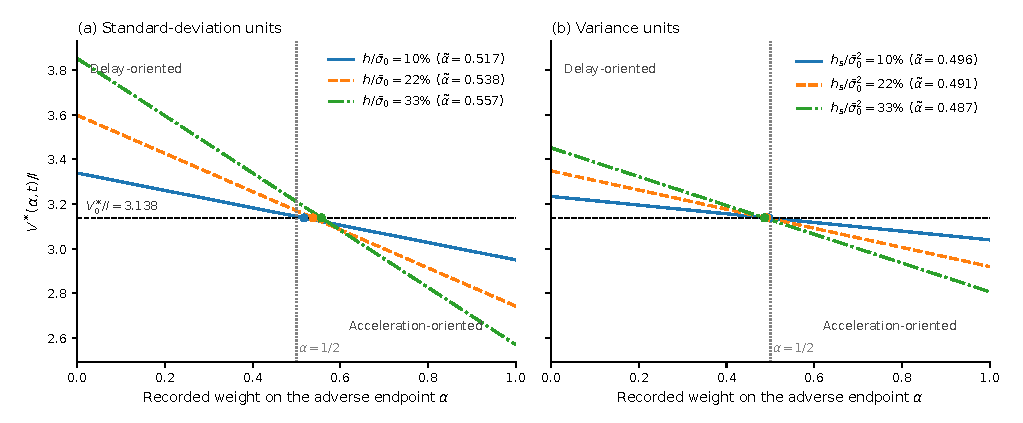
\includegraphics[width=0.9\textwidth]{figures/fig2_trigger_ratio.pdf}
\caption{Trigger ratio $V^{*}/I$ across recorded weights at three ambiguity radii. Directional labels indicate shifts from the no-ambiguity anchor. Panel (a) declares the ambiguity set in standard-deviation units. Panel (b) declares the same relative radius in variance units. Markers show the critical weight of each curve. The trigger is convex in $\sigma_p$ and concave in $\sigma_p^{2}$. The critical weight therefore lies above one half in panel (a) and below one half in panel (b).}
\label{fig:ratio}
\end{figure*}

\subsection{Price relevance of the contested-price interval}

The classification implied by the member triggers is read on the price axis. Converting each member trigger $V^{*}(\alpha_i,t)$ to the carbon-price scale gives the marginal carbon-price threshold
\begin{equation}
P^{*}_{i}=\frac{V^{*}(\alpha_i,t)\,\delta}{Q},\qquad \delta=r-\mu_c,
\label{eq:price}
\end{equation}
where $\delta$ is the net discount margin. $Q$ denotes annual captured emissions. It equals the annual CO$_2$ output of the plant multiplied by the capture rate assumed by \citet{Sun2024}. Eq.~(\ref{eq:price}) equates the trigger with the present value $P^{*}Q/\delta$ of perpetual carbon-price-linked cash flows. The no-ambiguity threshold $P^{*}_{0}:=\Vzero\delta/Q$ is called the anchor threshold. Eq.~(\ref{eq:price}) applies a positive common factor, so the thresholds inherit the critical weight defined on triggers. Define the contested-price interval and its width as
\begin{equation}
\begin{aligned}
C_t&:=\Bigl[\min_i P^{*}_{i},\;\max_i P^{*}_{i}\Bigr),\\
B_t&:=\mathrm{width}(C_t)=\max_i P^{*}_{i}-\min_i P^{*}_{i}.
\end{aligned}
\label{eq:interval}
\end{equation}
The recorded weight vector $\{\alpha_i\}$ is the weight profile of the gate. For $h_t>0$, $P^{*}(\alpha)$ is affine and strictly decreasing. Two profiles with the same extreme weights therefore yield the same interval at a fixed positive radius. The gap between the two endpoint triggers is $2V^{*\prime}(\sbar)h_t+O(h_t^{3})$. To leading order, the width factorizes as
\begin{equation}
B_t\approx 2\,(\alpha_{\max}-\alpha_{\min})\,V^{*\prime}(\sbar)\,h_t\,\frac{\delta}{Q}.
\label{eq:width}
\end{equation}
This approximation reproduced the exact width within 0.06\% over the primary radius range. The width is thus approximately the product of three factors. These are the recorded-weight range, the ambiguity radius, and the local trigger sensitivity in price units, $2V^{*\prime}(\sbar)\delta/Q$. At $h_t=0$, the width is zero, and no price produces a mixed classification. A change in the weight of one member moves an edge only when it changes the smallest or the largest recorded weight. The width then changes as well. The price-relevance condition uses the full min-max interval of Eq.~(\ref{eq:interval}).

\paragraph{Price-relevance condition} At a gate, let $P_t$ denote the prevailing effective carbon price, called the prevailing price. The classification rule assigns member $i$ an invest classification when $P_t\ge P^{*}_{i}$ and a wait classification otherwise. Both classifications occur among members if and only if
\begin{equation}
P_t\in C_t\iff \min_i P^{*}_{i}\le P_t<\max_i P^{*}_{i}.
\label{eq:relevance}
\end{equation}
Outside $C_t$, all members receive the same classification, even with distinct thresholds.

\paragraph{Basis of the threshold} The comparison between the prevailing price and the member thresholds is meaningful only on a stated threshold basis. $P^{*}$ is a marginal carbon-price threshold under the stated cash-flow mapping. It excludes operating costs, the energy penalty, transport and storage costs, and subsidies. Excluded costs are properties of the project, and members differ only in their recorded weights. An excluded cost expressible as a common per-tonne adjustment therefore shifts every member threshold equally.

\paragraph{Common adjustments} Two adjustments of practical interest act identically on every member threshold through different operations. A common per-tonne cost or subsidy shifts all thresholds by the same amount. With the perpetual trigger ratios held fixed, replacing the perpetuity with a common finite-horizon annuity multiplies all thresholds by the same factor. Both adjustments are monotone and preserve the equality between a member threshold and the anchor threshold. The member ordering and the critical weight therefore stay unchanged, while the classification at a fixed prevailing price may move. The shift leaves the interval width and the absolute threshold error of the affine rule unchanged. The factor rescales both, so the error stays unchanged only in relative terms.

Let $s$ denote a common per-tonne subsidy and $c$ a common per-tonne cost, both constant across members, and define $\Delta=c-s$. Every member threshold becomes $P^{*}_{i,\mathrm{obs}}=P^{*}_{i}+\Delta$, and the interval $C_t=[L,U)$ becomes $[L+\Delta,\,U+\Delta)$. A state-dependent or quantity-dependent component requires a different project-value specification.

\paragraph{Member-specific adjustments} An adjustment varying across members changes the interval width by at most the spread of the adjustments. It can also reverse the member ordering and break the single equality defining the critical weight.

\subsection{Trigger formulations and the accuracy of the affine rule}

Table~\ref{tab:formulations} lists the affine rule and three alternative trigger formulations. All except the equilibrium of \citet{HuangYu2021} are evaluated numerically. The pre-commitment $\aMEU$ optimum serves as the accuracy benchmark. The recursive $\alpha$-mixture of the generator serves as an analytical comparator. Here, $\Vlin(\alpha)$ denotes the member trigger of Eq.~(\ref{eq:affine}), and $\VMEU(\alpha,V_0)$ denotes the benchmark optimum at the same recorded weight.

\subsubsection{The pre-commitment benchmark}

For a trigger $V^{*}$ and a reference project value $V_0<V^{*}$, let $\tau$ denote the first hitting time of $V^{*}$. The standard real-options expression gives
\begin{equation}
\mathbb{E}_{\sigma}\bigl[e^{-r\tau}(V_{\tau}-I)\bigr]=\Bigl(\frac{V_0}{V^{*}}\Bigr)^{\beta_1(\sigma)}(V^{*}-I).
\label{eq:hitting}
\end{equation}
At this step, the ambiguity set is the pair of constant-volatility measures indexed by the declared endpoints. The factor $(V_0/V^{*})^{\beta_1}$ decreases in $\beta_1$ when $V_0<V^{*}$, and $\beta_1(\sigma)$ decreases in $\sigma$. The infimum and supremum of Eq.~(\ref{eq:hitting}) over the set are therefore attained at $\slow$ and $\shigh$, respectively. No admissible calibration reverses this endpoint ordering. A reversal would require a reference value above the trigger, or an exercise payoff nonlinear enough to make the project value decrease in volatility. The $\aMEU$ objective for a trigger rule is
\begin{multline}
J^{\alpha}(V^{*},V_0)=(V^{*}-I)\\
\times\biggl[\alpha\Bigl(\frac{V_0}{V^{*}}\Bigr)^{\beta_1(\slow)}+(1-\alpha)\Bigl(\frac{V_0}{V^{*}}\Bigr)^{\beta_1(\shigh)}\biggr].
\label{eq:Jalpha}
\end{multline}
The optimal trigger $\VMEU(\alpha,V_0)\equiv\arg\max_{V^{*}}J^{\alpha}(V^{*},V_0)$ has no closed form for $\alpha\in(0,1)$. Bounded scalar optimization computes it. Solving this scalar problem at each recorded weight yields the benchmark member-threshold vector. The maximization runs over constant triggers. The solution is therefore optimal within the class of constant-threshold rules under the pre-commitment criterion.

The benchmark vector depends on the reference project value $V_0$. The pre-commitment objective is evaluated directly at this value, without a recursive value function. The benchmark is defined for $V_0$ below the benchmark trigger of every member, a region called the benchmark domain. We fix $V_0=I$, the value at which immediate investment just breaks even. This value lay in the domain at every evaluated cell. A cell entered the evaluation only when $V_0$ lay below the low-endpoint trigger $\Vlow$. By Proposition~\ref{prop:benchmark}(i), this is a conservative sufficient form of the domain condition. Both calculations use the same economic primitives, volatility endpoints, recorded weights, and radius grid.

Table~\ref{tab:formulations} arranges the four formulations by role. The recursive $\alpha$-mixture shares two features with the affine rule, a closed form and independence from the reference value. The benchmark serves as the comparator at the same reporting granularity, a member-indexed threshold vector. It is required whenever the affine-only release rule fails. The equilibrium of \citet{HuangYu2021} completes the table.

Two conditions qualify the benchmark vector as the accuracy standard. The computed maximizer must be global, and its position relative to the affine trigger must be known. Proposition~\ref{prop:benchmark} settles both through one quantity, the spread between the two endpoint exponents.

\begin{proposition}[Benchmark well-posedness and one-sidedness]\label{prop:benchmark}
Write $\blo:=\beta_1(\slow)$ and $\bhi:=\beta_1(\shigh)$ for the exponents at the two endpoints, and $\Db:=\blo-\bhi>0$ for their spread. Fix a recorded weight $\alpha$ and a reference project value $V_0$ in the benchmark domain.
\begin{enumerate}
\item[(i)] Unique global maximizer. Every stationary point of $J^{\alpha}$ lies in $[\Vlow,\Vhigh]$. If
\begin{equation}
\Db\le 1\quad\text{or}\quad(\Db-1)\,\Vhigh\le\Db\,\Vlow,
\label{eq:unique}
\end{equation}
the stationary point is unique and is the global maximizer. Condition~(\ref{eq:unique}) is free of $\alpha$ and of $V_0$.
\item[(ii)] One-sidedness. Assume Condition~(\ref{eq:unique}). For $\alpha\in(0,1)$,
\begin{equation}
\Vlin(\alpha)\ge\VMEU(\alpha,V_0)\iff\frac{\blo-1}{\bhi-1}\ge\Bigl(\frac{\Vlin(\alpha)}{V_0}\Bigr)^{\Db}.
\label{eq:onesided}
\end{equation}
The affine and benchmark triggers coincide at the endpoint weights $\alpha=0$ and $\alpha=1$. Since $\Vlin$ decreases in $\alpha$, replacing it by $\Vhigh$ yields a condition sufficient for every recorded weight at once. At $V_0=I$, the condition holds whenever $\Db\le1$.
\end{enumerate}
\end{proposition}

Both conditions have closed forms in the calibration and the radius. A gate can therefore check them without solving the benchmark. Condition~(\ref{eq:unique}) held at all 33 admissible calibrations across the admissible radius range, with a slack of at least $0.906I$. The global-maximizer property therefore held for every reported benchmark value. A separate scan covered 30,090 cells defined by calibration, radius, reference value, and weight. It counted exactly one interior maximum of $J^{\alpha}$ in every cell. The same counter flagged a deliberately bimodal control function. Condition~(\ref{eq:onesided}) held at all 33 calibrations and every registered radius up to 22\%. At the 33\% stress radius, it failed at one calibration, with $r=0.12$, $\mu_c=0.02$, and $\sbar=0.199$. There, the affine trigger fell below the benchmark for recorded weights near 0.01. The relative gap was at most $4.5\times10^{-6}$, confirmed at 40-digit precision. This failure lay above the 10\% cap, where the release rule already requires a dual report.

\begin{table*}[!t]
\caption{Decision-rule outputs and their roles in this paper.}
\label{tab:formulations}
\centering
\footnotesize
\renewcommand{\arraystretch}{1.15}
\begin{tabular}{@{}L{0.17\textwidth}L{0.25\textwidth}L{0.14\textwidth}L{0.36\textwidth}@{}}
\toprule
Formulation & Type of output & Dynamic consistency & Role in this paper\\
\midrule
Affine endpoint rule, Eq.~(\ref{eq:affine}) & Member-trigger map $\alpha_i\mapsto V^{*}_{i}(t)$. Eqs.~(\ref{eq:price}) and (\ref{eq:interval}) convert it to $\{P^{*}_{i}\}$, $C_t$, and $B_t$ & Not applicable (static gate-reporting map) & Closed-form mechanism, independent of the reference value, preserving member thresholds\\
Pre-commitment $\aMEU$ optimum, Eq.~(\ref{eq:Jalpha}) & Member-trigger vector dependent on $V_0$, evaluated at $\{\alpha_i\}$ & No (pre-commitment rule) & Direct comparator, benchmark available by recomputation at any gate, and required fallback\\
Recursive $\alpha$-mixture of the generator, Eq.~(\ref{eq:effvar}) & Member-trigger vector $V^{*}(\sigma_{\mathrm{eff}}(\alpha_i))$, independent of $V_0$, with a unique scalar boundary & Yes, by construction & Third comparator. Its critical weight has the closed form of Eq.~(\ref{eq:critrec}) and lies above one half. The variance mixture fixes this value for any increasing trigger map\\
Time-consistent $\aMEU$ equilibrium \citep{HuangYu2021} & Member-indexed equilibrium stopping regions. Scalar boundaries apply only when uniquely defined in a common state & Yes & On the constant-endpoint set of this paper, the recursive row is time-consistent with a single-threshold stopping region, as a threshold report requires. Under state-dependent prior sets, compressing the regions into $\{P^{*}_{i}\}$ is inadmissible\\
\bottomrule
\end{tabular}
\end{table*}

\subsubsection{The recursive alternative}

The pre-commitment objective is evaluated once, at the gate. Applying the same $\alpha$-mixture at every state yields a rule dynamically consistent by construction. In this setting, the rule also has a closed form. Under convexity of the continuation value, the generator collapses to the ordinary geometric Brownian form at the effective variance
\begin{equation}
\sigma^{2}_{\mathrm{eff}}(\alpha)=\alpha\,\slow^{2}+(1-\alpha)\,\shigh^{2}.
\label{eq:effvar}
\end{equation}
The recursive trigger is then $V^{*}_{\mathrm{rec}}(\alpha)=V^{*}(\sigma_{\mathrm{eff}}(\alpha))$. It is free of any reference project value. Solving $\sigma_{\mathrm{eff}}(\tilde{\alpha})=\sbar$ gives the critical weight
\begin{equation}
\tilde{\alpha}_{\mathrm{rec}}(h)=\frac{1}{2}+\frac{h}{4\sbar},
\label{eq:critrec}
\end{equation}
which exceeds one half at every positive radius.

Convexity also makes the effective variance state-independent, so the recursive problem reduces to the ordinary stopping problem at this variance. Its stopping region is bounded by a single threshold. A time-consistent formulation thus meets the reporting condition in this setting. The recursive columns of Table~\ref{tab:threeform} report the implied critical weight and interval width. The recursive rule serves as a comparator because mixing the two generators mixes variances. A recorded weight then indexes an effective volatility. Under the affine rule, the weight indexes a position between the two endpoint triggers.

Eqs.~(\ref{eq:critrec}) and (\ref{eq:kappa}) locate the difference between the two rules. The recursive displacement is $h/(4\sbar)$. Its coefficient of $h$ equals the geometric term of the curvature ratio. The affine coefficient also retains a negative $\beta$-curvature correction. Near the anchor, the affine critical weight therefore lies below the recursive one. Table~\ref{tab:threeform} compares all three formulations, and this ordering held at every evaluated radius. The affine and recursive critical weights lay above one half. The pre-commitment critical weight at $V_0=I$ lay below one half and decreased in the radius. Under the benchmark at this reference value, both the sign of Corollary~\ref{cor:global} and the monotonicity of Corollary~\ref{cor:mono} reverse. At the baseline calibration and the four-member reference profile, the widths differed far less than the labels. At a 10\% radius, the widths were 10.945\,CNY/t (affine), 11.027\,CNY/t (recursive), and 10.717\,CNY/t (pre-commitment). The two comparators lay within 2.1\% of the affine width. This distance grew with the radius and reached 6.4\% at the 33\% stress radius. This magnitude was close to the 6.15\% maximum trigger error over all calibrations and the full radius grid.

The closed forms in Eqs.~(\ref{eq:critical}) and (\ref{eq:critrec}) both rest on the perpetual geometric Brownian structure. Eq.~(\ref{eq:critrec}) requires a convex continuation value, so the generator collapses to Eq.~(\ref{eq:effvar}). The displacement in Eq.~(\ref{eq:critical}) requires $V^{*}(\sigma_p)$ to be convex in $\sigma_p$. A different price process can break either property. The ratio in Eq.~(\ref{eq:critical}) was therefore recomputed under three further specifications. These were a finite investment horizon, a mean-reverting log price, and a jump diffusion. Each specification is solved on one grid shared by the three volatility endpoints. The discretization bias in the trigger level then largely cancels in the ratio. Table~\ref{tab:departures} reports the binding cells. The critical weight stayed above one half in all 52 evaluated cells, with a smallest value of 0.5080. At a 25-year option horizon, it differed from its perpetual value by at most 0.0020. Under jumps, the continuation value is no longer a power function of $V$, and the GBM closed form for Eq.~(\ref{eq:critical}) is unavailable. The ratio in Eq.~(\ref{eq:critical}) still defines the critical weight when the specification yields two ordered scalar endpoint triggers. Three steps then supply the required trigger values. First, the two endpoint triggers must exist and remain ordered. Second, the trigger must be monotone and curved in the declared coordinate. Third, the weight equating the affine threshold with the anchor threshold is recomputed from the new continuation value. The jump row of Table~\ref{tab:departures} follows these three steps numerically.

\begin{table*}[!t]
\caption{Critical weight under three departures from the perpetual geometric Brownian specification.}
\label{tab:departures}
\centering
\footnotesize

\begin{tabular}{@{}llcccc@{}}
\toprule
 & & \multicolumn{4}{c}{Smallest $\tilde{\alpha}$ at $h/\sbar$}\\
\cmidrule(l){3-6}
Specification & Auxiliary grid & 5\% & 10\% & 22\% & 33\%\\
\midrule
Perpetual GBM (reference) & None & 0.5086 & 0.5171 & 0.5378 & 0.5570\\
Finite investment horizon & $T=5$--80 years & 0.5082 & 0.5172 & 0.5376 & 0.5565\\
Mean-reverting log price & $\kappa=0$--0.30 & 0.5080 & 0.5170 & 0.5375 & 0.5566\\
Jump diffusion & $\phi=0$--0.50 & 0.5085 & 0.5170 & 0.5375 & 0.5566\\
\bottomrule
\end{tabular}
\par\smallskip
\parbox{\columnwidth}{\footnotesize\emph{Notes.} Each entry is the smallest critical weight over the auxiliary grid at the given radius, which binds the above-one-half claim. The finite-horizon grid carries six horizons, the mean-reversion grid four reversion speeds, and the jump grid three variance shares. In the mean-reversion and jump grids, one of these settings is a solver control. The three grids give 24, 16, and 12 cells. On the jump grid, the no-jump control bound at every radius, because moving declared variance into jumps raised the critical weight. On the mean-reversion grid, the $\kappa=0$ control bound at the 10\%, 22\%, and 33\% radii. A positive reversion speed raised the critical weight at these radii. At the 5\% radius, $\kappa=0.30$ bound by 0.0005. The perpetual row is the exact affine value of Eq.~(\ref{eq:critical}). Each departure is solved by the Crank-Nicolson method. The three volatility endpoints share one logarithmic grid within each departure, so the level bias cancels in the ratio. The free boundary is interpolated between nodes.}
\end{table*}

\begin{table*}[!t]
\caption{Critical weight and interval width under different $h/\sbar$ settings and the three trigger formulations.}
\label{tab:threeform}
\centering
\footnotesize
\begin{tabular}{@{}lcccccc@{}}
\toprule
 & \multicolumn{3}{c}{Critical weight $\tilde{\alpha}$} & \multicolumn{3}{c}{$B_t$ (CNY/t)}\\
\cmidrule(lr){2-4}\cmidrule(l){5-7}
$h/\sbar$ & Affine & Recursive & Pre-commitment & Affine & Recursive & Pre-commitment\\
\midrule
5\% & 0.5086 & 0.5125 & 0.4980 & 5.473 & 5.494 & 5.415\\
10\% & 0.5171 & 0.5250 & 0.4960 & 10.945 & 11.027 & 10.717\\
22\% & 0.5378 & 0.5550 & 0.4920 & 24.069 & 24.442 & 22.999\\
33\% & 0.5570 & 0.5825 & 0.4898 & 36.073 & 36.861 & 33.775\\
\bottomrule
\end{tabular}
\par\smallskip
\parbox{0.95\textwidth}{\footnotesize\emph{Notes.} Baseline calibration and four-member reference profile. The recursive column is the closed form $1/2+\rho/4$ of Eq.~(\ref{eq:critrec}), which numerical evaluation reproduced to 14 decimal places. The pre-commitment columns are evaluated at $V_0=I$. Only the pre-commitment output depends on this reference value, and only its critical weight fell below one half.}
\end{table*}

\subsubsection{Accuracy of the affine rule}

Proposition~\ref{prop:accuracy} separates the size of the trigger error from the location of the critical weight.

\begin{proposition}[Local trigger approximation and critical-weight sensitivity]\label{prop:accuracy}
At the reference project value $V_0=I$, fix a recorded weight $\alpha\in[0,1]$.
\begin{enumerate}
\item[(i)] First-order agreement. The affine and benchmark triggers both expand about the anchor volatility as $\Vzero+(1-2\alpha)V^{*\prime}(\sbar)h+O(h^{2})$. Hence $\Vlin-\VMEU=O(h^{2})$.
\item[(ii)] Quadratic trigger-error expansion. The relative trigger error satisfies $\lvert\Vlin-\VMEU\rvert/\VMEU=C(\alpha)(h/\sbar)^{2}+O\bigl((h/\sbar)^{3}\bigr)$, where $C(\alpha)=K\alpha(1-\alpha)$ for a positive calibration-dependent constant $K$. The leading coefficient is largest at $\alpha=\frac{1}{2}$ and vanishes at the endpoint weights.
\item[(iii)] Separation of magnitude and location. At a positive radius, the critical weight is defined by $V^{*}(\tilde{\alpha},h)=\Vzero$. The ratio of the $O(h^{2})$ curvature term to the $O(h)$ slope determines its distance from $1/2$. Part (i) puts the trigger discrepancy at order $h^{2}$. The critical weights of the two formulations, however, differ at first order, $\tilde{\alpha}_{\mathrm{lin}}-\tilde{\alpha}_{\alpha\text{-MEU}}=O(h)$.
\end{enumerate}
\end{proposition}

The local constant in Proposition~\ref{prop:accuracy}(ii) is $K=\sbar^{2}\Psi_I/\Vzero$, where $\Psi_I$ is the second-order benchmark-curvature term. $K$ equaled 1.0495 at the baseline calibration.

The position of the benchmark critical weight relative to one half depends on the reference project value. Over the baseline grid, the benchmark critical weight fell on both sides of one half. It exceeded one half only for reference values below roughly $0.83I$ at a 5\% radius and $0.87I$ at 33\%. By Corollary~\ref{cor:global}, the affine critical weight exceeds one half everywhere. On the evaluated grid, the two never coincided at a positive radius. At $V_0=I$, they straddled one half. A member with $\alpha_i=1/2$ was therefore delay-oriented under the affine rule and acceleration-oriented under the benchmark. The band of weights with opposite labels widened with the radius and the reference value. At $V_0=I$, its width ran from 0.011 at a 5\% radius to 0.067 at the 33\% stress radius. At $V_0=0.5I$, it ran from 0.003 to 0.018.

Parts (i) and (ii) of Proposition~\ref{prop:accuracy} characterize the trigger-level error. This error does not pass to the interval width unchanged. Each member trigger carries an absolute error of $O(h^{2})$ and a relative error of $O((h/\sbar)^{2})$. The width is only $O(h)$ when the extreme weights differ. Its absolute error is $O(h^{2})$, or $O(h^{3})$ when the extreme weights are symmetric about one half. Without this symmetry, the relative width error is $O(h/\sbar)$.

The directional labels depend on the location of the critical weight, which leads to two reporting rules. First, a label is released only with the reference project value and the declared ambiguity coordinate. Under the benchmark, the side of one half depends on the reference value. Under the affine rule, it depends on the coordinate. Second, a label is de-emphasized when the recorded weight of the member lies within the illustrative $\pm0.05$ review band around the critical weight. Elicitation noise alone can move such a weight across the critical weight. In a perturbation test, independent errors with standard deviation 0.05 were added to a ten-member Beta(5,\,5) profile. The interval width stayed centered near its noiseless value, with a coefficient of variation of 12.9\%. The label-flip probability for the weights nearest the critical weight reached 47.6\%. At every radius admitted by the release rule, the review band contained the whole opposite-label band. A member whose label depends on the formulation therefore already receives a de-emphasized label. The contested-price interval and the invest-or-wait classification depend on the member thresholds and fall under a separate safeguard.

Table~\ref{tab:accuracy} reports the finite-radius approximation error at the baseline calibration with $V_0=I$. On the primary radius range, the maximum relative member-trigger error was 1.26\%. This corresponded to at most 1.47\,CNY/t in the marginal carbon-price threshold. On the extended range, the maximum reached 2.82\%. The 33 admissible economic calibrations form a 36-point Cartesian grid minus three cells violating $r>\mu_c$. Across them, the maxima rose to 2.74\% on the primary range and 6.15\% on the full grid. The interval-width error for the four-member reference profile was also computed at the largest radius of the reconstructed signal path. It was at most 2.25\% across the tested reference values. Figure~\ref{fig:errormap} maps the relative trigger error over the full grid of radii and weights at the baseline calibration.

The dependence of the benchmark vector on $V_0$ affects the directional labels. Fixing $V_0=I$ removes this dependence only through a second reporting choice. The affine rule needs no such choice, since it uses only the two endpoint triggers and the recorded weights. For reference values from $0.75I$ to $1.25I$, the reported affine interval stayed unchanged. The benchmark interval departed from it by at most 0.28\,CNY/t inside the release cap. The gate outcome agreed under both rules at every sampled value. The affine report is therefore released, and the benchmark serves as the accuracy standard and the fallback. The release envelopes were constructed and audited against the benchmark.

\begin{table}[!t]
\caption{Accuracy of the affine rule against the numerically computed $\aMEU$ benchmark.}
\label{tab:accuracy}
\centering
\scriptsize
\setlength{\tabcolsep}{3.5pt}
\begin{tabular}{@{}cccccc@{}}
\toprule
$h/\sbar$ & $\alpha$ & $\Vlin/I$ & $\VMEU/I$ & \makecell{Abs. rel.\\err. (\%)} & \makecell{Signed $\Delta P^{*}$\\(CNY/t)}\\
\midrule
0.10 & 0.25 & 3.241 & 3.235 & 0.19 & $+0.23$\\
0.10 & 0.50 & 3.144 & 3.136 & 0.26 & $+0.31$\\
0.10 & 0.75 & 3.047 & 3.041 & 0.20 & $+0.23$\\
0.22 & 0.25 & 3.384 & 3.355 & 0.85 & $+1.07$\\
0.22 & 0.50 & 3.170 & 3.131 & 1.25 & $+1.47$\\
0.22 & 0.75 & 2.956 & 2.926 & 1.02 & $+1.12$\\
0.33 & 0.25 & 3.531 & 3.470 & 1.77 & $+2.30$\\
0.33 & 0.50 & 3.211 & 3.124 & 2.76 & $+3.24$\\
0.33 & 0.55 & 3.147 & 3.060 & 2.81 & $+3.23$\\
0.33 & 0.75 & 2.890 & 2.824 & 2.36 & $+2.50$\\
\bottomrule
\end{tabular}
\par\smallskip
\parbox{\columnwidth}{\scriptsize\emph{Notes.} Relative errors are unsigned magnitudes. The signed difference is $\Delta P^{*}=P^{*}_{\mathrm{lin}}-P^{*}_{\alpha\text{-MEU}}$. A positive value indicates a higher marginal carbon-price threshold under the affine rule. The rows show a subset of the $\alpha$ grid. Over the whole grid, the baseline maxima were 1.26\% on the primary range and 2.82\% on the full range. Both were attained at weights between the tabulated rows.}
\end{table}

\begin{figure}[!t]
\centering
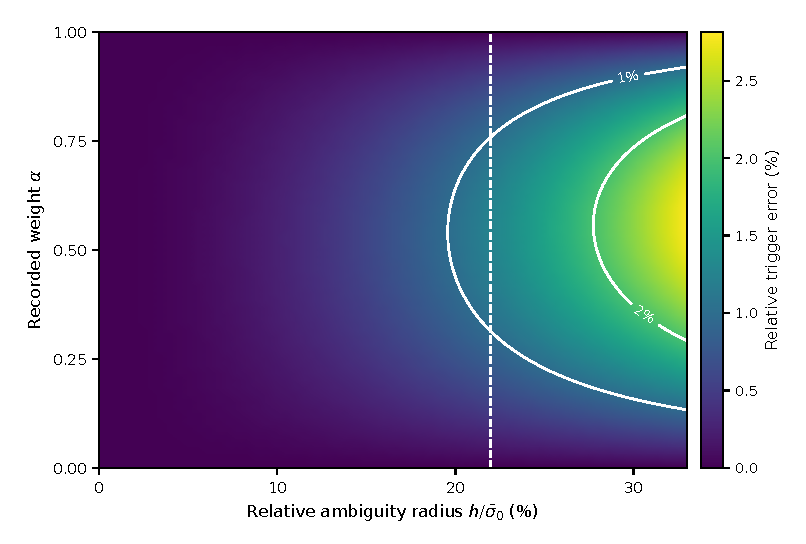
\includegraphics[width=\columnwidth]{figures/fig3_error_map.pdf}
\caption{Relative trigger error of the affine rule against the numerically computed $\aMEU$ benchmark. The grid covers ambiguity radius $h/\sbar$ and recorded weight $\alpha$ at the baseline calibration and $V_0=I$. Shading shows the relative trigger error in percent. White contours mark the 1\% and 2\% levels. The dashed vertical line marks $h/\sbar=22\%$, the upper bound of the primary radius range. The error peaked near $\alpha=1/2$ and vanished at the endpoint weights, consistent with Proposition~\ref{prop:accuracy}(ii).}
\label{fig:errormap}
\end{figure}

\subsection{Classification fidelity and information retained by member thresholds}

\subsubsection{Classification fidelity}

Small trigger errors can still change classifications when a price lies between the affine and benchmark thresholds. The comparison is therefore made on the price axis, vector against vector. Two quantities are computed for each configuration. The first is the intersection over union (IoU) of the affine and benchmark contested-price intervals. The second is the omitted mixed share, the length of the benchmark interval outside the affine interval divided by the benchmark width. For prices in this omitted region, the affine rule reports a unanimous classification unsupported by the benchmark. These geometric diagnostics require no price distribution.

The criteria are evaluated on a fixed deterministic design. The design combines the 33 admissible calibrations with four panel sizes (3, 5, 7, and 9) and six recorded-weight profiles. It uses relative radii of 5\%, 10\%, 15\%, and 22\%. The reference project value equals the investment cost. The design contains 3,168 configurations.

Criterion C1 requires at least 95\% of configurations to attain an IoU of at least 0.90. Criterion C2 requires the 95th percentile of the omitted mixed share to be at most 5\%. Both criteria concern the tail of the distribution. On the full set, 89.5\% of configurations attained an IoU of at least 0.90, below the 95\% required by C1. The 95th percentile of the omitted mixed share was 7.65\%, above the C2 limit. The full set therefore met neither criterion. At the 10\% radius alone, 98.2\% of configurations met the IoU requirement. On the pooled 5\% and 10\% set, this share was 99.1\%, and the 95th percentile of the omitted mixed share was 4.15\%. Both criteria held on this restricted set.

\subsubsection{Information retention}

Criteria C1 and C2 test whether the affine interval reproduces the benchmark interval. A separate simulation examined whether the member-threshold vector retains price-axis information lost by any single trigger. It compares the affine member-threshold vector with single-trigger compressions of the benchmark vector. The simulation generates 2,000 panels for each combination of five radii, four panel sizes, and five weight families. Each simulated panel draws one of the 33 calibrations. The design contains 200,000 panels, 160,000 of them within the primary radius range.

Member-vector loss is the mean absolute price-axis distance between each affine threshold and its benchmark counterpart. It is expressed as a percentage of the anchor threshold. Four single-trigger candidates enter the comparison. They are the anchor threshold, the benchmark thresholds at the mean and median recorded weights, and the largest benchmark member threshold. The loss of a candidate is computed by replacing every affine threshold with the candidate threshold. For each panel, a restricted ex post comparator selects the candidate with the lowest loss. It uses the benchmark vector after the panel is generated. The comparison therefore runs against the most favorable of the four candidate summaries in hindsight.

Criterion C3 has two parts. The median member-vector loss must be at most one half of the median loss of the comparator. The 95\% design-cell resampling interval for the improvement must also exclude zero. The four primary radii, four panel sizes, and five weight families define 80 design cells. Each cell contributes the median paired loss difference within it.

Across the in-range panels, the median member-vector loss was 0.224\% of the anchor threshold. The median loss of the comparator was 1.944\%, a reduction of 88.5\%. The member-threshold vector had the lower loss in 99.5\% of the panels. The experiment quantifies the price-axis information lost when a benchmark vector with $m$ members is compressed to one threshold.

The comparator selected the median-weight benchmark threshold in every tested panel, as the absolute-distance loss implies for odd panel sizes. Across the 80 design cells, the median cell-level loss difference was 1.65\% of the anchor threshold. Its 95\% resampling interval ran from 1.31\% to 2.06\%, so Criterion C3 was met.

A second question concerns how much of this gain requires the full vector. A separate deterministic grid, equal in size to the fidelity evaluation set, addressed it. A three-threshold summary reported the smallest, median, and largest benchmark thresholds. It cut the median loss to 0.502\% of the anchor threshold. The best single trigger reached 2.240\%, and the member-threshold vector reached 0.235\%. The full vector thus removed 53\% of the loss left by the three-threshold summary. It was the more accurate of the two in 72.5\% of configurations. Three-member panels form a quarter of this grid. There, the three-threshold summary reproduces the benchmark vector exactly. The comparison is informative only on the remaining cells. Adding a min-max midpoint and a quartile-based composite to the comparator set left the ordering unchanged. Most of the improvement over a single trigger therefore came from reporting more than one threshold. The member-indexed vector also identifies the member behind each threshold, which a sorted summary cannot do.

Table~\ref{tab:simulation} reports the Monte Carlo results by radius, and each row summarizes 40,000 simulated panels. Its omitted-share percentiles differed from the deterministic statistics because the simulation drew random weight profiles.

The same panels supply two inputs for an institution setting its own criteria. The first input is a length in price units, the omitted mixed share multiplied by the benchmark width. Table~\ref{tab:simulation} reports this length normalized by the anchor threshold. It ran from 0.09\% at a 5\% radius to 3.60\% at the stress radius. At the anchor threshold, these values equaled about 0.10 and 4.24\,CNY/t. The second input is panel dependence. Fidelity improved monotonically with panel size and degraded under one-sided weight skew. A skewed profile brings the two interval edges closer together. A given trigger displacement then removes a larger share of the benchmark interval. The weakest cell was a three-member panel under skew. A committee can compare these lengths with the price band over which it regards the gate decision as open. It can then set its own release cap.

A three-member panel under skew is visible at the gate without the benchmark. A dispersion statistic of the recorded weights might therefore serve as an escalation rule. The natural candidate is the ratio of the full interval width to its interquartile counterpart. This ratio failed as an escalation rule. For three-member panels, this ratio equals two for every profile. Classification fidelity for these panels ranged from 48.5\% to 99.2\%, measured as the share of configurations with an IoU of at least 0.90. For larger panels, the correlation between the ratio and fidelity stayed below 0.25. The weight shape and the panel size did separate passing cells from failing cells, and a gate records both. The release rule nonetheless conditions on price-axis distances, because its proximity conditions catch the affected gates directly.

The four-member application profile was evaluated separately and deterministically. The evaluation used 30 direct comparisons between the affine rule and the benchmark, over five radii and six reference values. These checks and the 32 archived-price cells of Table~\ref{tab:margins} are archived in the replication package.

\begin{table*}[!t]
\caption{Classification fidelity and price-axis information loss across simulated panels of sizes 3, 5, 7, and 9. The 33\% radius is a stress case.}
\label{tab:simulation}
\centering
\footnotesize
\begin{tabular}{@{}lL{0.17\textwidth}L{0.3\textwidth}L{0.33\textwidth}@{}}
\toprule
$h/\sbar$ & IoU, median (5th percentile) & 95th-percentile omitted mixed, benchmark share / anchor-normalized length (\%) & Median loss, member vector / four-candidate ex post comparator (\% of anchor threshold)\\
\midrule
5\% & 0.978 (0.929) & 4.0 / 0.09 & 0.039 / 0.862\\
10\% & 0.957 (0.862) & 7.9 / 0.35 & 0.156 / 1.720\\
15\% & 0.937 (0.801) & 11.7 / 0.78 & 0.350 / 2.601\\
22\% & 0.911 (0.723) & 16.8 / 1.65 & 0.735 / 3.810\\
33\% & 0.876 (0.621) & 23.9 / 3.60 & 1.573 / 5.746\\
\bottomrule
\end{tabular}
\end{table*}

\subsubsection{Finite-registry safeguard}

Within the tested design, the simulation supported retaining the member-threshold vector. Classification fidelity near the interval edges weakened as the radius grew. The loss was sharpest for skewed profiles and small panels. A release rule is therefore attached to the member-threshold report. Consider a registered calibration $\theta=(r,\mu_c,\sbar)$ and an evaluated radius $\rho=h/\sbar$. With $L_{\mathrm{lin}}$ and $U_{\mathrm{lin}}$ as the edges of the affine interval $C_t$, let
\begin{equation}
\begin{aligned}
\eR(\theta,\rho)&:=\max_{\alpha\in[0,1]}\frac{\lvert\Vlin(\alpha)-\VMEU(\alpha,I)\rvert}{\Vzero},\\
\ER(\theta,\rho)&:=P^{*}_{0}\,[\eR(\theta,\rho)+\varepsilon_{\mathrm{num}}],\\
\dedge&:=\min\{\lvert P_t-L_{\mathrm{lin}}\rvert,\;\lvert P_t-U_{\mathrm{lin}}\rvert\},\\
\dmember&:=\min_i\,\lvert P_t-P^{*}_{i,\mathrm{lin}}\rvert.
\end{aligned}
\label{eq:safeguard}
\end{equation}
The distance $\dedge$ protects the three-state gate summary of unanimous wait, mixed, or unanimous invest. The distance $\dmember$ protects the invest-or-wait label of every member. The interval edges are member thresholds, so $\dmember\le\dedge$, and the member condition binds. Both distances are retained for audit. The envelope contains the registered maximum member-trigger error plus a numerical tolerance. $\ER$ carries the anchor threshold $P^{*}_{0}$ as a multiplicative factor, with the tolerance inside the bracket. A common rescaling of the member thresholds therefore rescales $\ER$ by the same factor. The anchor-normalized trigger error stays invariant. The release decision can still change, because the prevailing price stays fixed while the thresholds rescale. The registry stores the dimensionless envelope $\eR$. After any revision of the investment cost or the captured volume, the gate recomputes $P^{*}_{0}$ and $\ER$. It then re-evaluates both proximity distances. The audit record carries $I/Q$ and $P^{*}_{0}$ with the registry identifiers. A past release can thus be reconstructed on its original price axis.

The benchmark may be requested at any gate, and the registry governs only its omission. Affine-only reporting requires four conditions. (i) The calibration and the canonical radius key are registered exactly. (ii) The radius is at most 10\%. (iii) The reference value satisfies $V_0/I=1$, the only value at which the release rule was evaluated. (iv) Both proximity distances exceed $\ER$. If any condition fails, or if the solver or envelope version is unregistered, the gate recomputes the benchmark and issues a dual report. The reporting interface passes the member-threshold vector and the fallback status. A match must come from the frozen serialized key. Rounded display values and values reparsed from the upstream signal file do not qualify. Interpolation is excluded, because no certified release envelope exists between evaluated radius keys. The cap is a hard cutoff, so a rounded configuration constant can fall on the wrong side of it. One low-radius scenario targeted exactly 10\% and yielded 10.30\% at its rounded constant, outside the affine-only region. Exact-key matching guards against this error. An institution may prespecify a rule mapping each gate radius to a registered key. The release guarantee then applies to the discretized ambiguity set. The audit record retains both the original radius and the registered radius.

When the benchmark is recomputed, the gate first evaluates the uniqueness condition~(\ref{eq:unique}). This sufficient condition guarantees a single stationary point of the benchmark objective. When it holds, the maximizer is the unique stationary point on $[\Vlow,\Vhigh]$, and a bounded solve suffices. When it fails, the gate isolates every stationary point. It then compares the objective at all of them and at both endpoints before releasing a benchmark classification. Condition~(\ref{eq:onesided}) is recorded separately, because it governs the one-sided reading of the dual report. Recomputation costs one bounded scalar solve per member. The algorithm fixes the number of solves, and the wall-clock time depends on the computing environment. In prospective institutional use, the registry should be append-only. Algorithm~\ref{alg:gate} states the matching, versioning, and solver rules.

The registry makes a released classification auditable after the fact. A registry cell is indexed by the economic calibration, the radius key, and the reference value. It carries the envelope version and the solver version. The gate audit record adds the recorded weights, the prevailing price, and the cost-to-volume inputs. A later reviewer can then identify the inputs behind a past classification. The reviewer can also recompute it without re-eliciting any weight. Under the append-only rule, a revised input opens a new dated cell. The earlier cell stays readable with its original guarantee. The rule also isolated the disagreement cells in the registry. Across the 3,960 registered configurations, the two formulations disagreed in 57 cells. None of these cells cleared the radius cap and both proximity conditions together. Two of the 57 lay at a 10\% radius, where a proximity flag caught them. The envelopes were constructed at all 3,960 domain-valid configurations with $V_0/I=1$, and two checks bounded their numerical error. A denser $\alpha$ grid detected no exceedance in the 165 calibration-radius cells. A second check compared the finite weight grid with a certified upper bound on the discrepancy over $[0,1]$ in each cell. This bound used a closed-form Lipschitz constant and a branch-and-bound search. It exceeded the grid maximum by at most $3.1\times10^{-6}$\,CNY/t and changed no release decision.

The 10\% cap follows from the deterministic fidelity evaluation. It is the largest evaluated radius at which both criteria held. A refinement at intermediate radii located the failure just above the cap. C2 failed first, at 11\%. There, the 95th percentile of the omitted mixed share reached 5.4\%, against the 5\% limit. At the 10\% radius, the same quantity was 4.96\%, so the binding radius passed C2 by 0.04 percentage points. The breach at 11\% was 0.4 percentage points, which suggests a gradual loss of accuracy across the cap. By Proposition~\ref{prop:accuracy}(i), raising the cap from 10\% to 22\% would multiply the leading error term by about five.

The cap was also tested on 18 calibrations and five weight profiles absent from the evaluated grid, with six calibrations outside its range. The release quantity behaved similarly on this held-out set. The largest within-cell member-threshold deviation had a 95th percentile across cells of 0.5141\,CNY/t on the held-out set. The corresponding value on the evaluated grid was 0.5143\,CNY/t. The normalized fidelity criteria were more sensitive to the weight profile. They held on four of the five held-out profiles. They failed on one profile with weights clustered within 0.06 of one half. For this profile, the benchmark interval shrank to 0.72\% of the anchor threshold. A similar absolute discrepancy then became a much larger relative one. IoU normalizes by the union of the two intervals, and the omitted mixed share normalizes by the benchmark width. Both registered this effect, although the absolute deviation stayed the same. For this reason, the release rule conditions on absolute price-axis distances.

Above the cap, the dual report is mandatory. The differences between the two rules there ran in one direction. Across the three larger radii and the weakest profiles, member-level classifications agreed in more than nine cases in ten. In no evaluated cell did the affine rule classify a price as invest while the benchmark classified it as wait. Proposition~\ref{prop:benchmark}(ii) explains this pattern. Under the one-sidedness condition, the affine report errs toward deferral. The condition held throughout the affine-only region.

Figure~\ref{fig:release} shows the release decision as a single pass over the four registered conditions. These conditions bound the member thresholds and thus the released classification. They bound the released interval width $B_t$ only in absolute terms, within $2\ER$. At the reference project value of the release rule, the width error for the four-member reference profile was 1.29\%. The larger 2.25\% figure came from other tested reference values, outside the release region. The width shrinks as the recorded weights cluster. On tightly clustered profiles, the same absolute error is therefore a larger fraction of the width. Input validity is checked on a separate branch. A failed upstream acceptance check blocks the threshold report.

The model results fall into two groups. The analytical group holds wherever the maintained model holds. A unique critical weight splits the members around the no-ambiguity anchor, and trigger curvature in the declared coordinate locates it relative to one half. The numerical group rests on a finite registry. The affine rule stayed close to the benchmark on the evaluated grid, yet small trigger errors could still change a classification. The release rule therefore ties affine-only reporting to registered configurations and price-axis distances. The practical relevance of these properties depends on the inputs of a specific project.

\begin{figure*}[!t]
\centering
\resizebox{0.97\textwidth}{!}{%
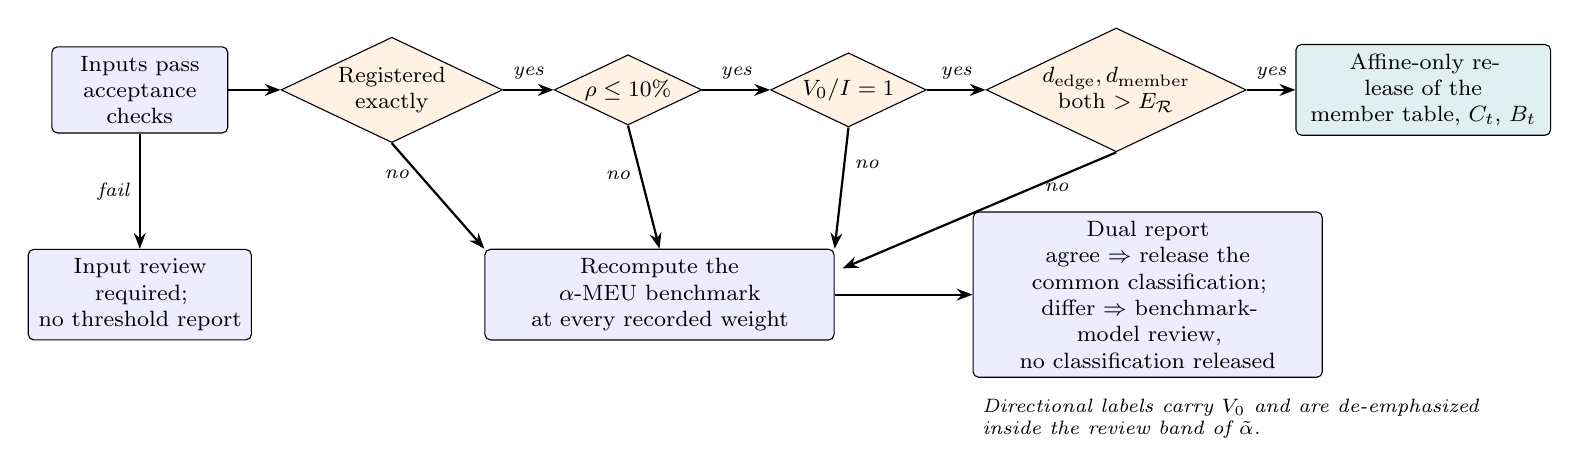
\begin{tikzpicture}[
  font=\footnotesize,
  proc/.style={draw, rounded corners=2pt, align=center, fill=blue!7, minimum height=0.9cm},
  dec/.style={draw, diamond, aspect=2.1, align=center, fill=orange!10, inner sep=1pt},
  ok/.style={draw, rounded corners=2pt, align=center, fill=teal!12, minimum height=0.9cm},
  arr/.style={-{Stealth[length=2mm]}, thick},
  lab/.style={font=\scriptsize\itshape}
]
\node[proc, text width=2.0cm] (in) at (0,0) {Inputs pass acceptance checks};
\node[dec] (reg) at (3.2,0) {Registered\\exactly};
\node[dec] (rad) at (6.2,0) {$\rho\le10\%$};
\node[dec] (v0) at (9.0,0) {$V_0/I=1$};
\node[dec] (dist) at (12.4,0) {$\dedge,\dmember$\\both $>\ER$};
\node[ok, text width=3.0cm] (aff) at (16.3,0) {Affine-only release of the\\member table, $C_t$, $B_t$};
\node[proc, text width=2.6cm] (rev) at (0,-2.6) {Input review required;\\no threshold report};
\node[proc, text width=4.2cm] (rec) at (6.6,-2.6) {Recompute the $\aMEU$ benchmark\\at every recorded weight};
\node[proc, text width=4.2cm] (dual) at (12.8,-2.6) {Dual report\\agree $\Rightarrow$ release the\\common classification;\\differ $\Rightarrow$ benchmark-model review,\\no classification released};
\draw[arr] (in) -- (reg);
\draw[arr] (reg) -- node[lab, above]{yes} (rad);
\draw[arr] (rad) -- node[lab, above]{yes} (v0);
\draw[arr] (v0) -- node[lab, above]{yes} (dist);
\draw[arr] (dist) -- node[lab, above]{yes} (aff);
\draw[arr] (in) -- node[lab, left]{fail} (rev);
\draw[arr] (reg.south) -- node[lab, left, pos=0.3]{no} (rec.north west);
\draw[arr] (rad.south) -- node[lab, left, pos=0.4]{no} (rec.north);
\draw[arr] (v0.south) -- node[lab, right, pos=0.3]{no} (rec.north east);
\draw[arr] (dist.south) -- node[lab, right, pos=0.3]{no} ($(rec.north east)+(0.1,-0.25)$);
\draw[arr] (rec) -- (dual);
\node[lab, align=left, anchor=north west] at ($(dual.south west)+(0,-0.15)$) {Directional labels carry $V_0$ and are de-emphasized\\inside the review band of $\tilde{\alpha}$.};
\end{tikzpicture}}
\caption{Release decision for one gate. The gate first verifies the registered input acceptance checks, and a failure blocks the threshold report. Four registered conditions are then checked in sequence. The calibration and radius key must be registered exactly. The relative radius must be at most 10\%. The reference project value must satisfy $V_0/I=1$. Both $\dedge$ and $\dmember$ must exceed the registered envelope $\ER$. Passing all four conditions releases the affine-only report with the member-threshold vector, $C_t$, and $B_t$. Failing any condition routes the gate to a dual report, with the $\aMEU$ benchmark recomputed at every recorded weight. Both member tables are issued in this mode. A gate-level classification is released only when the two three-state summaries agree, and individual member assignments may still differ. A discrepancy triggers a benchmark-model review, with no precedence for either rule.}
\label{fig:release}
\end{figure*}

\section{Illustrative numerical application to a 600-MW CCUS retrofit}

A 600-MW coal-fired CCUS retrofit supplies such project inputs. The application uses four inputs. The first is the economic calibration with the project inputs. The second is an ambiguity radius from a date-reconstructed policy-text signal. The third and fourth are a four-member reference profile of recorded weights and the archived price series. The construction returns member thresholds and quarterly contested-price intervals. Daily China Emission Allowance (CEA) prices are compared with the corresponding quarterly intervals, and each archived price is classified retrospectively. The anchor, corpus, and encoder are fixed ex post. For example, the volatility anchor estimated on 2024 and 2025 data applies to the entire historical signal path. Sensitivity checks varied the profiles, inputs, anchors, and scaling constants.

\subsection{Numerical setting and policy-text signal}

\subsubsection{Corpus and signal construction}

The corpus comprises 682 central-government energy and climate policy records. Four bodies issued these records. They are the National Development and Reform Commission, the National Energy Administration, the State Council, and the Ministry of Ecology and Environment. Of these records, 678 fell inside the analysis window from 2016Q1 to 2025Q4. The records were retrieved from the PKULaw database, which assigns each one a stable document number.

The retrieval targeted the years 2016 to 2025. A thematic screen retained records classified under energy, climate, carbon markets, or emissions trading, based on source tags and a title keyword filter. A document-type screen kept substantive plans, notices, guidance, and formal responses. It excluded press releases, routine administrative notices without policy content, and non-Chinese texts.

The dispersion signal is quarterly, so incorrect document dates distort its path. Dates in the database may differ from official issuance dates. An audit therefore matched each record to an official agency page where possible. It resolved such a page for 414 of the 682 records. Two date assignments were compared. The reference assignment uses the date printed in each archived record and is reproducible from the archive alone. The page-date assignment uses a verified agency page date where available and the printed date otherwise. The two assignments produced different paths for the quarterly signal and the interval width. Four records bear 2015 printed dates and fall outside the window, so they are excluded. Four other records carry month-only dates. A month identifies the quarter, and these four records lie inside the window and are retained.

Each document is represented by precomputed layer-14 embeddings from the Qwen3-0.6B model \citep{Yang2025}. The embeddings are pooled across subword tokens with term frequency-inverse document frequency (TF-IDF) weights and normalized to unit length. This primary representation, Qwen3-L14, was fixed before the signal was compared with realized volatility. The policy-semantic-dispersion index is
\begin{equation}
\PSDI_t=1-\lVert\bar{c}_t\rVert,
\label{eq:psdi}
\end{equation}
where $\bar{c}_t$ is the centroid of all normalized document vectors in period $t$. A larger $\PSDI_t$ indicates greater dispersion around the period centroid. The signal tracks temporal variation in dispersion through the rolling four-quarter standard deviation
\begin{equation}
w_t=\mathrm{std}_4(\PSDI_t,\PSDI_{t-1},\PSDI_{t-2},\PSDI_{t-3}).
\label{eq:wt}
\end{equation}
Here $\mathrm{std}_4$ is the population standard deviation, with divisor four, over the current and previous three quarters. Figure~\ref{fig:architecture} writes this window as $\PSDI_{t:t-3}$.

Six alternative dispersion statistics on the same vectors moved the peak quarter in two cases. None of them changed the gate outcome. One corpus-composition check moved both the peak quarter and the peak width. Excluding documents longer than 2,000 characters before truncation retained 384 of the 678 records. The peak quarter shifted from 2024Q4 to 2023Q1, and the peak interval width rose from 6.63 to 8.59\,CNY/t. The Spearman rank correlation between this length-filtered path and the reference path was 0.61. One of two replacement encoders also moved the peak. MacBERT-base placed the peak in 2019Q2 at a width of 5.42\,CNY/t. Its quarterly signal had a Spearman rank correlation of 0.305 with the reference.

\subsubsection{Screening procedure and input diagnostics}

Algorithm~\ref{alg:gate} summarizes the gate update from the registered radius source through the release rule to the reported object. Its cost depends on the radius source. With a declared radius, the affine branch is $O(m)$ in the panel size $m$. With the text-derived radius, it is $O(\lvert D_t\rvert+m)$ once the embeddings exist, where $\lvert D_t\rvert$ is the number of documents in period $t$. This count assumes a fixed embedding dimension and a four-quarter history. The fallback adds one benchmark optimization per member. One release envelope on the 2,001-point weight grid took about 0.2 seconds per calibration-radius cell. This wall-clock figure varies with machine load.

The proportional map $h_t=c_w w_t$ requires a nonnegative signal, since $h_t$ is a radius. The rolling standard deviation is nonnegative by construction. The reference configuration sets the scaling constant $c_w$ to one. The ambiguity radius then equals the signal before the admissibility cap. Before the national emissions trading scheme (ETS), the lagged signal showed a positive but imprecise association with realized volatility. During the national ETS period, the estimated slope changed sign. Over the 18 quarters of this period, the slope was $-18.07$, with a 95\% confidence interval of $[-34.57,-1.57]$. The interval for the shorter estimation window spanned zero. Neither subsample identified a stable value for $c_w$. Five further diagnostics covered directional association, temporal-order permutation, construct validity, an event-style check, and national ETS stability. None of them supported a stable mapping. The series therefore serves as a scenario input configuring the radius.

The signal was also compared with an established policy-uncertainty measure, the log China Economic Policy Uncertainty (EPU) index of \citet{Baker2016}. Over 2017 to 2024, the Pearson correlation was 0.265 ($n=32$), with a four-lag heteroskedasticity and autocorrelation consistent (HAC) $p$-value of 0.036. Over the 14 national ETS quarters covered by the EPU sample, it was 0.264. Slope estimates distinguishable from zero still left the scale open. Propagating the pre-ETS slope to the thresholds gave a width envelope of up to 19.2\,CNY/t. This value was about 2.9 times the configured peak width of 6.63\,CNY/t. The pre-ETS slope and the national ETS slope differed by 61.08, with a standard error of 30.94. The 95\% interval for this difference, based on the $t$ distribution with 23 Welch degrees of freedom, contained zero. The data therefore did not fix even the direction of a rescaling. A mapping re-estimated on the national ETS window explained none of the out-of-sample variation in 2024 and 2025.

Two properties suit this series to its illustrative role. First, an institution can archive and re-encode the documents. With the corpus, encoding pipeline, and scaling convention recorded, a past radius can be recomputed without re-eliciting any expert input. Second, the documents come from the same regulatory process whose ambiguity the gate considers.

Two calibration routes could replace the convention with an estimate. A forward-looking route would set the endpoints from option-implied volatility bounds. This route requires a traded allowance option, and the national market had none over the sample period. A survey route would use the forecast dispersion elicited from allowance-price forecasters with a documented track record. Each source would need its own validation and an explicit mapping to the declared radius. Combining the two would need an aggregation rule for their overlapping information.

For prospective use, an institution should set a calibration cutoff and use only information available by this date. Before later gate outcomes are observed, it should also register several items. These are a target radius $h_{\mathrm{ref}}$ and a strictly positive reference signal $w_{\mathrm{ref}}$. They also include the volatility-anchor window, the encoder version, the admissibility cap, and the review cadence. The scaling constant is then $c_w=h_{\mathrm{ref}}/w_{\mathrm{ref}}$. The target radius, achieved radius, rounded display value, and canonical registry key are distinct fields. Release matching follows the exact-key rule. Under exact matching, an unseen radius triggers benchmark recomputation. Prospective affine-only use therefore requires a radius discretization declared in advance or a release envelope certified over a continuous radius interval. Later gate outcomes do not retune $c_w$ or the reference statistic. A documented drift or regime review opens a new dated configuration under the append-only rule. A stable forward-volatility series may later support statistical calibration. The institution should then prespecify training and holdout windows and register the fitted map as a new configuration.

\begin{algorithm*}[!t]
\caption{Gate-level member thresholds and safeguarded classification.}
\label{alg:gate}
\footnotesize
\begin{algorithmic}[1]
\Require One registered radius source, either a declared radius $h_t$ (or $\rho_t$) or the application-specific text construction with its registered pipeline identifiers
\Require Dated deployment record for $\sbar$, $c_w$, $\epsilon$, the registered price-recording buffer $b$, and registry-versioning requirements
\Require Recorded weights $\{\alpha_i\}_{i=1}^{m}\in[0,1]^{m}$ passing the prespecified input-acceptance checks \Comment{reporting inputs}
\Require $r>\mu_c>0$, $I,Q>0$, prevailing price $P_t$, and benchmark reference $V_0$ inside the benchmark domain
\Require Versioned finite registry snapshot $\mathcal{R}^{(\nu)}$ with frozen canonical serialized configuration identifiers
\Require Direct-benchmark request flag $b_{\mathrm{direct}}\in\{0,1\}$
\Ensure Affine member table, $\tilde{\alpha}$, $C_t$, $B_t$, released classification, audit record, and reporting mode
\Ensure Benchmark table on fallback or direct request
\State initialize $\eR$, $\ER$, both proximity flags, and both certification flags to \emph{not evaluated} \Comment{filled when the lookup or check runs}
\If{the deployment record, economic, or recorded-weight checks fail}
  \State \Return input review required; issue no threshold report
\EndIf
\If{the registered radius source is a declared radius}
  \State read the registered $h_t$ or $\rho_t$
\Else
  \State obtain $h_t$ by the application-specific text construction; Eqs.~(\ref{eq:psdi}) and (\ref{eq:wt}) give $\PSDI_t$ and $w_t$, and the admissibility cap gives $h_t$ \Comment{application-specific step}
\EndIf
\State \textbf{Analytical layer.} $\rho_t\gets h_t/\sbar$; $(\sigma_{-},\sigma_0,\sigma_{+})\gets(\sbar-h_t,\sbar,\sbar+h_t)$
\State solve Eq.~(\ref{eq:char}) at $(\sigma_{-},\sigma_0,\sigma_{+})$ and compute $(\Vlow,\Vzero,\Vhigh)$
\If{$V_0\ge\Vlow$}
  \State \Return input review required; issue no threshold report \Comment{benchmark-domain check}
\EndIf
\State $V^{*}_{i}\gets\alpha_i\Vlow+(1-\alpha_i)\Vhigh$ for all $i$
\State $\tilde{\alpha}\gets1/2$ if $h_t=0$; otherwise $\tilde{\alpha}\gets(\Vhigh-\Vzero)/(\Vhigh-\Vlow)$
\State \textbf{Interface layer.} $P^{*}_{0}\gets\Vzero(r-\mu_c)/Q$; $P^{*}_{i}\gets V^{*}_{i}(r-\mu_c)/Q$ for all $i$; $C_t\gets[\min_iP^{*}_{i},\max_iP^{*}_{i})$; $B_t\gets\max_iP^{*}_{i}-\min_iP^{*}_{i}$
\State affine summary $\gets\textsc{classify}(P_t,\{P^{*}_{i}\})$ \Comment{three-state gate summary}
\State $\dedge\gets\min\{\lvert P_t-\min_iP^{*}_{i}\rvert,\lvert P_t-\max_iP^{*}_{i}\rvert\}$; $\dmember\gets\min_i\lvert P_t-P^{*}_{i}\rvert$
\State buffer-flag $\gets[\min\{\dedge,\dmember\}<b]$ \Comment{price-input diagnostic reported beside the classification}
\State $(k_{\theta},k_{\rho},k_{V})\gets\textsc{canonical\_ids}(r,\mu_c,\sbar,\rho_t,V_0/I)$
\State registered $\gets\textsc{registry\_lookup}(k_{\theta},k_{\rho},k_{V};\mathcal{R}^{(\nu)})$ \Comment{exact values; no rounded match or interpolation}
\If{registered}
  \State read the dimensionless registered envelope $\eR$, the grid maximum recorded for the cell \Comment{$I$ and $Q$ enter only through $P^{*}_{0}$}
  \State $\ER\gets P^{*}_{0}[\eR+\varepsilon_{\mathrm{num}}]$; near-edge $\gets[\dedge\le\ER]$; near-member $\gets[\dmember\le\ER]$
  \State fallback $\gets b_{\mathrm{direct}}\lor[V_0/I\neq1]\lor[\rho_t>0.10]\lor$ near-edge $\lor$ near-member
\Else
  \State both proximity flags $\gets$ not evaluated; fallback $\gets$ true
\EndIf
\If{fallback}
  \State global-certified $\gets$ Condition~(\ref{eq:unique}) holds at $(\theta,\rho_t)$
  \If{global-certified}
    \State solve Eq.~(\ref{eq:Jalpha}) on $[\Vlow,\Vhigh]$ at $(\alpha_i,V_0)$ for all $i$
  \Else
    \State isolate every stationary point of Eq.~(\ref{eq:Jalpha}) on $[\Vlow,\Vhigh]$ and compare the objective at all of them and at both endpoints
    \If{no global maximizer is certified}
      \State \Return benchmark-model review required; issue no released classification
    \EndIf
  \EndIf
  \State one-sided-certified $\gets$ Condition~(\ref{eq:onesided}) holds at $(\theta,\rho_t)$ \Comment{governs the one-sided reading only}
  \State convert the benchmark triggers by Eq.~(\ref{eq:price})
  \State mode $\gets$ dual report
  \If{the affine and benchmark three-state summaries agree}
    \State released classification $\gets$ this summary \Comment{agreement concerns the summary; member assignments may differ, and both member tables are released}
  \Else
    \State released classification $\gets$ none; benchmark-model review required \Comment{no priority for either rule}
  \EndIf
\Else
  \State released classification $\gets$ affine summary; mode $\gets$ affine-only report
\EndIf
\State record the audit fields $I/Q$, $P^{*}_{0}$, $\eR$, and $\ER$, the radius source, the two certification flags, and the mode
\State \Return affine member table, $C_t$, $B_t$, $\tilde{\alpha}$, released classification, $(\nu,k_{\theta},k_{\rho},k_{V})$, the audit record, and the benchmark table on fallback or direct request
\end{algorithmic}
\end{algorithm*}

\subsection{Baseline setting}

Table~\ref{tab:calibration} lists the baseline calibration for the 600-MW retrofit. The investment cost and annual captured emissions follow \citet{Sun2024}. The discount rate follows the Chinese national appraisal standard \citep{NDRC2006}. The annual carbon-price growth scenario is set to 0.04. The volatility anchor is the annualized standard deviation of 474 within-market log returns. These returns come from 475 daily national CEA closing prices in 2024 and 2025. The Shanghai pilot and national CEA data are separate series, so no return spans the market boundary. The annualized estimate was 0.249. No liquid CEA options market existed over the sample period, so this historical estimate serves as the forward-volatility anchor.

Table~\ref{tab:costcontext} places the anchor threshold beside external capture-cost references for context. The anchor threshold was 117.7\,CNY/t, and a demonstration reference lies near 250\,CNY/t. $P^{*}$ is a marginal threshold, and the references are technology costs. The common-adjustment identity gives the amount a committee adds to the reported basis before comparing the two. Table~\ref{tab:translation} evaluates this identity at illustrative values of $\Delta$ spanning these references. In a hypothetical accounting scenario with $\Delta=250$\,CNY/t, the interval moved to $[363.38,\,370.01)$\,CNY/t. A committee comparing against a figure with these components reads the gate at this adjusted level.

The cost adjustment enters the thresholds additively, and the calibrated inputs $I$ and $Q$ enter multiplicatively. By Eqs.~(\ref{eq:trigger}) and (\ref{eq:price}), every $P^{*}_{i}$ is proportional to $I$ and inversely proportional to $Q$. A different cost or captured-volume assumption is therefore a common-factor adjustment. The trigger-to-cost ratios stay unchanged, because $V^{*}$ is proportional to $I$ and independent of $Q$. The threshold levels, the interval width, and the price-unit envelope rescale with the common factor. The classification at a fixed prevailing price may move with them. Both inputs may carry considerable appraisal uncertainty. The reconstructed reference path peaked in 2024Q4 at a radius of 6.057\% of the volatility anchor. At this radius, the baseline lower interval edge was 113.38\,CNY/t. This edge lay above the highest archived price of 105.65\,CNY/t. A 10\% reduction in $I/Q$ moved the edge to 102.04\,CNY/t. The same archived price then entered the interval, and the gate became mixed. A 20\% reduction moved the edge to 90.70\,CNY/t and placed the price above the whole interval. The critical weight and the member ordering stayed unchanged in all these cases.

\begin{table*}[!t]
\caption{Baseline calibration for the 600-MW CCUS numerical application.}
\label{tab:calibration}
\centering
\footnotesize
\begin{tabular}{@{}L{0.26\textwidth}L{0.07\textwidth}L{0.16\textwidth}L{0.42\textwidth}@{}}
\toprule
Parameter & Symbol & Value & Source or basis\\
\midrule
Investment cost & $I$ & $1.585\times10^{9}$\,CNY & \citet{Sun2024}\\
Discount rate & $r$ & 0.08 & NDRC and Ministry of Construction (2006)\\
Annual carbon-price growth scenario & $\mu_c$ & 0.04 & Decision-analysis input, varied in the sensitivity analysis\\
Carbon-price volatility anchor & $\sbar$ & 0.249 & National CEA daily closing prices traded on the Shanghai Environment and Energy Exchange, 2024 to 2025 (475 prices)\\
Annual captured emissions & $Q$ & $1.69\times10^{6}$\,t/yr & \citet{Sun2024}\\
Admissibility margin & $\epsilon$ & 0.5 & Fixed cap parameter, nonbinding in the reference application\\
Signal-to-radius scaling constant & $c_w$ & 1.0 & Fixed reference convention\\
\bottomrule
\end{tabular}
\end{table*}

\begin{table*}[!t]
\caption{External cost context for the marginal carbon-price threshold $P^{*}$.}
\label{tab:costcontext}
\centering
\footnotesize
\begin{tabular}{@{}L{0.26\textwidth}L{0.2\textwidth}L{0.47\textwidth}@{}}
\toprule
Reference quantity & Reported value & Interpretation\\
\midrule
This paper, no-ambiguity marginal carbon-price threshold & $\approx117.7$\,CNY/t & Marginal carbon-price threshold implied by the option trigger. It excludes capture OPEX, the energy penalty, transport, storage, and subsidies.\\
China coal-power CCUS demonstration reference & $\approx250$\,CNY/t & Reported capture-cost reference for the Taizhou coal-fired carbon-capture facility of China Energy \citep{YangX2023}. Technology-cost figure.\\
IEA dilute-stream capture-cost reference & More than USD 40/t, and more than USD 100/t in some cases & Capture-cost range reported by \citet{IEA2020} for dilute CO$_2$ streams in power generation and blast-furnace steelmaking.\\
\bottomrule
\end{tabular}
\end{table*}

\begin{table*}[!t]
\caption{Common per-tonne cost translation of the member thresholds at the reference-peak radius.}
\label{tab:translation}
\centering
\footnotesize
\begin{tabular}{@{}lccccc@{}}
\toprule
Scenario & \makecell{$\Delta$\\(CNY/t)} & \makecell{Lower edge\\(CNY/t)} & \makecell{Upper edge\\(CNY/t)} & \makecell{$B_t$\\(CNY/t)} & \makecell{Margin to $P_{\max}$\\(CNY/t)}\\
\midrule
No common adjustment (reported basis) & 0 & 113.38 & 120.01 & 6.63 & $+7.73$\\
Illustrative low common cost & 150 & 263.38 & 270.01 & 6.63 & $+157.73$\\
Illustrative cost at the Taizhou reference level & 250 & 363.38 & 370.01 & 6.63 & $+257.73$\\
Illustrative high common cost & 350 & 463.38 & 470.01 & 6.63 & $+357.73$\\
Illustrative cost at the Taizhou level, net of an 80\,CNY/t subsidy & 170 & 283.38 & 290.01 & 6.63 & $+177.73$\\
\bottomrule
\end{tabular}
\par\smallskip
\parbox{0.95\textwidth}{\footnotesize\emph{Notes.} The first row is the basis of every other result in this paper. The remaining rows apply the common-adjustment identity. The $\Delta$ values are illustrative settings spanning the external references of Table~\ref{tab:costcontext}. $P_{\max}$ is the highest archived national CEA closing price, 105.65\,CNY/t. The final column is the lower edge minus $P_{\max}$, and a positive value means every member classifies this price as wait. The identity holds for adjustments common across members and constant per tonne.}
\end{table*}

\subsection{Screening outputs under alternative component configurations}

Table~\ref{tab:components} compares four component configurations under a common economic calibration. The first two configurations yield a single trigger and no member-level dispersion. The third introduces member-level dispersion with the relative radius fixed at 10\% of the volatility anchor. Its interval width is therefore the same at every gate. The full method updates the interval at every gate. Its quarterly widths ranged from 1.67 to 6.63\,CNY/t under the reference scaling convention.

\begin{table*}[!t]
\caption{Screening outputs under alternative component configurations.}
\label{tab:components}
\centering
\footnotesize
\begin{tabular}{@{}L{0.27\textwidth}L{0.11\textwidth}L{0.15\textwidth}L{0.1\textwidth}L{0.25\textwidth}@{}}
\toprule
Configuration & Text-derived radius & Heterogeneous recorded weights & $B_t$ (CNY/t) & Output at each gate\\
\midrule
Conventional real-options baseline ($h=0$) & No & No & 0 & Single trigger\\
Homogeneous $\alpha=0.5$ & Yes & No & 0 & Single trigger\\
Fixed $h$ ($h/\sbar=10\%$, static) & No & Yes & 10.945 & Fixed interval; classification evaluated at each gate\\
Full method ($c_w=1.0$, time-varying) & Yes & Yes & 1.67 to 6.63 & Time-varying interval and classification summary\\
\bottomrule
\end{tabular}
\end{table*}

\subsection{Member-level interpretability at a review gate}

The reconstructed path stayed below the 10\% release cap, so its intervals were narrower than at the cap. Across the 37 quarterly gates, the relative radius ran from 1.524\% to 6.057\%. The cap bound at none of them. Exact key matching was the binding constraint. The 2024Q4 peak radius was a registered key, and the other 36 gate radii were not. The release rule therefore sent these 36 gates to benchmark recomputation. With a radius discretization registered in advance, an institution rounds all 37 radii to registered keys at or below the cap. Table~\ref{tab:members} fixes the relative radius at the cap, the upper limit of affine-only eligibility, and reports member triggers and thresholds. The reference profile contains four equally spaced recorded weights from 0.25 to 1. These weights are design inputs for the illustration.00. Its weight range of 0.750 was the widest among five profiles compared at a common radius. Under the affine, strictly decreasing map, it therefore produced the largest interval width among the five. The weight $\alpha=0.50$ lay just below the critical weight. The affine rule labeled this weight delay-oriented by a narrow margin, and the benchmark labeled it acceleration-oriented. The thresholds barely moved across formulations. At the reference-peak radius, the affine, recursive, and pre-commitment widths were 6.630, 6.660, and 6.545\,CNY/t. The latter two differed from the reported width by $+0.46\%$ and $-1.27\%$. A gate may therefore read the thresholds first and treat the directional label as secondary.

\begin{table}[!t]
\caption{Member-specific trigger values and ambiguity premiums at the baseline economic calibration with $h_t/\sbar=10\%$.}
\label{tab:members}
\centering
\scriptsize
\setlength{\tabcolsep}{3pt}
\begin{tabular}{@{}lcccl@{}}
\toprule
Case & $V^{*}/I$ & $P^{*}$ (CNY/t) & AP$/I$ & Shift relative to anchor\\
\midrule
No-ambiguity anchor & 3.138 & 117.7 & 0 & Baseline\\
$\alpha=0.25$ & 3.241 & 121.6 & $+0.104$ & Delay-oriented\\
$\alpha=0.50$ & 3.144 & 118.0 & $+0.007$ & Delay-oriented\\
$\alpha=0.75$ & 3.047 & 114.3 & $-0.091$ & Acceleration-oriented\\
$\alpha=1.00$ & 2.950 & 110.7 & $-0.188$ & Acceleration-oriented\\
\bottomrule
\end{tabular}
\par\smallskip
\parbox{\columnwidth}{\scriptsize\emph{Notes.} AP$/I$ is the ambiguity premium divided by the investment cost. The final column labels the shift of each trigger relative to the anchor trigger. The ambiguity premium changed sign at the critical weight, 0.517 at this radius and calibration. The reconstructed radius stayed below 10\%, and the lower interval edge decreases with the radius. The value 110.7\,CNY/t is therefore a lower bound for the lower edge along the reconstructed reference path.}
\end{table}

\subsection{Dynamic intervals and archived-price classification under the reference configuration}

Figure~\ref{fig:dynamic} lets the radius vary across review gates and shows the contested-price interval under the reference configuration. The volatility anchor stays fixed at its estimated value, so all width variation comes from the reconstructed radius path. The shaded band lies between the two extreme member thresholds. The width reached 6.63\,CNY/t in 2024Q4. The reconstruction applies the anchor retrospectively. An as-of anchor, estimated only from prices available at each gate, could be computed at 14 gates. Over these gates, the peak quarter and the unanimous-wait outcome stayed unchanged. The lower panel compares the observed daily CEA price with the lower interval edge on the same time axis.

\begin{figure*}[!t]
\centering
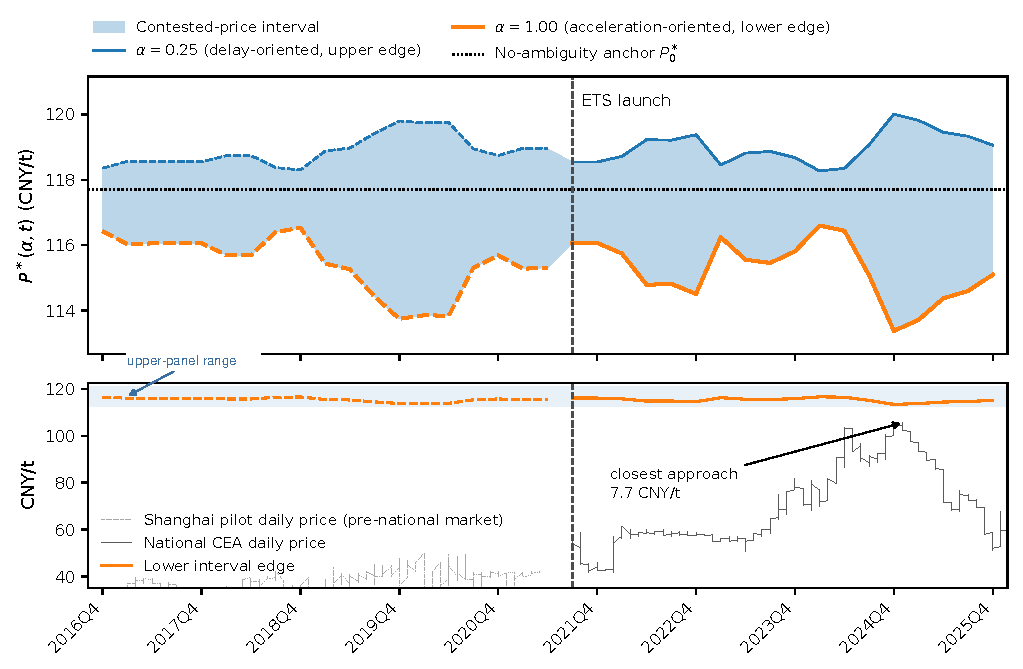
\includegraphics[width=0.9\textwidth]{figures/fig5_dynamic_interval.pdf}
\caption{Retrospective fixed-anchor reconstruction of the contested-price interval for the four-member reference profile. Dashed threshold segments mark the period before the national ETS, and solid segments mark the national ETS period. The vertical dashed line marks the ETS launch, and the horizontal dotted line marks the anchor threshold. The lower panel plots archived daily prices from two markets. The dotted series is the Shanghai pilot price before the national market, and the solid series is the national CEA price. The closest-approach annotation compares the lower edge with the national CEA observations only. On the reported path, the lowest lower edge and the highest archived price both fell in 2024Q4. This difference is therefore the contemporaneous closest approach.}
\label{fig:dynamic}
\end{figure*}

\subsubsection{Archived-price classification}

Under the reference configuration, $\Delta=0$, and the prevailing price equals the archived CEA price. Across the 1,073 daily CEA observations from 2021Q3 to 2025Q4, both the affine rule and the $\aMEU$ benchmark returned unanimous wait. The two rules share the lower interval edge by construction, since the reference profile includes the endpoint weight $\alpha=1$. The highest archived price, 105.65\,CNY/t, lay 7.73\,CNY/t below the lowest member threshold along the reconstructed path. The reference configuration is therefore a nonbinding baseline. Retaining the member-threshold vector and its interval therefore left the three-state classification unchanged along this price path. Changing the radius alone, or one economic primitive alone, produced binding configurations. Of 32 sensitivity configurations evaluated against the same price record, 15 placed the highest archived price at or above the lower edge. Ten of these were released as mixed and four as unanimous invest. The remaining one went to benchmark-model review because the two rules disagreed.

\subsection{Calibration sensitivity and safeguard behavior}

The sensitivity configurations perturb the baseline calibration, and the archived price history is the same in each. Any change in classification therefore comes from the threshold side.

\subsubsection{Worked gate reports}

Table~\ref{tab:worked} renders two cells of the 32-cell design as complete gate reports. These two cells exercise the two branches of the release rule. Both use the lower volatility anchor $\sbar=0.199$, the four-member reference profile, and $V_0=I$. They differ only in the evaluated radius.

In Configuration A, the radius was the frozen reference peak, and the interval was 4.56\,CNY/t wide. Its upper edge lay 0.002\,CNY/t below the prevailing price. All four members classified this price as invest, and the gate was unanimous. The member with the smallest recorded weight holds the upper edge, so the edge margin equals the nearest-member distance. This distance of 0.002\,CNY/t was far below the registered envelope of 0.059\,CNY/t. The proximity conditions failed, and the gate issued a dual report after benchmark recomputation. The benchmark placed the upper threshold at 105.60\,CNY/t, against an affine value of 105.65\,CNY/t, and the price cleared both. The conservative proximity rule fired, although the recomputation confirmed unanimous investment. In Configuration B, at the 10\% radius, the interval widened to 7.53\,CNY/t and contained the unchanged prevailing price. Three members classified the price as invest. The member with the smallest recorded weight classified it as wait, so the gate was mixed. Both proximity distances rose to 1.092\,CNY/t, against an envelope of 0.160\,CNY/t. The affine-only report was released.

In this pair, the wider interval eased release, because the test depends on the distance from the prevailing price to the nearest threshold. Widening carried the upper threshold past the price.

\begin{table*}[!t]
\caption{Worked reports for two cells of the 32-cell robustness design, both at the $\sbar=0.199$ calibration.}
\label{tab:worked}
\centering
\footnotesize
\begin{tabular}{@{}lcccc@{}}
\toprule
 & \multicolumn{2}{c}{Configuration A ($\rho=6.057\%$)} & \multicolumn{2}{c}{Configuration B ($\rho=10\%$)}\\
\cmidrule(lr){2-3}\cmidrule(l){4-5}
Report field & Affine & Benchmark & Affine & Benchmark\\
\midrule
\multicolumn{5}{@{}l}{\emph{Member-specific marginal carbon-price thresholds $P^{*}_{i}$ (CNY/t)}}\\
$\alpha_i=0.25$ & 105.65 & 105.60 & 106.74 & 106.62\\
$\alpha_i=0.50$ & 104.13 & 104.07 & 104.23 & 104.07\\
$\alpha_i=0.75$ & 102.61 & 102.56 & 101.73 & 101.60\\
$\alpha_i=1.00$ & 101.09 & 101.09 & 99.22 & 99.22\\
\multicolumn{5}{@{}l}{\emph{Interval, prevailing price, and classification}}\\
Critical weight $\tilde{\alpha}$ (affine) & \multicolumn{2}{c}{0.510} & \multicolumn{2}{c}{0.517}\\
Lower edge of $C_t$ (CNY/t) & 101.09 & 101.09 & 99.22 & 99.22\\
Upper edge of $C_t$ (CNY/t) & 105.65 & 105.60 & 106.74 & 106.62\\
Width $B_t$ (CNY/t) & 4.56 & 4.51 & 7.53 & 7.41\\
Prevailing price $P_t$ (CNY/t) & \multicolumn{2}{c}{105.65} & \multicolumn{2}{c}{105.65}\\
Members classified invest & 4 of 4 & 4 of 4 & 3 of 4 & 3 of 4\\
Gate state & unanimous invest & unanimous invest & mixed & mixed\\
\multicolumn{5}{@{}l}{\emph{Release rule of Eq.~(\ref{eq:safeguard}), evaluated on the affine report}}\\
$\dedge$ (CNY/t) & \multicolumn{2}{c}{0.002} & \multicolumn{2}{c}{1.092}\\
$\dmember$ (CNY/t) & \multicolumn{2}{c}{0.002} & \multicolumn{2}{c}{1.092}\\
Registered envelope $\ER$ (CNY/t) & \multicolumn{2}{c}{0.059} & \multicolumn{2}{c}{0.160}\\
\makecell[l]{Price-date sensitivity flag, margin below\\the 1.97\,CNY/t buffer (diagnostic only)} & \multicolumn{2}{c}{unresolved by price record} & \multicolumn{2}{c}{unresolved by price record}\\
Proximity flags & \multicolumn{2}{c}{edge, member} & \multicolumn{2}{c}{none}\\
Reporting mode & \multicolumn{2}{c}{dual report} & \multicolumn{2}{c}{affine-only}\\
Released classification & \multicolumn{2}{c}{unanimous invest} & \multicolumn{2}{c}{mixed}\\
\bottomrule
\end{tabular}
\par\smallskip
\parbox{0.95\textwidth}{\footnotesize\emph{Notes.} The calibration is $r=0.08$, $\mu_c=0.04$, and $\sbar=0.199$, at the reference value $V_0=I$ and the four-member reference profile. $P_t$ is the highest archived national CEA closing price over 2021Q3 to 2025Q4. Configuration A uses the frozen archived canonical serialized radius key, and its displayed value is rounded for this table only. The upper edge of Configuration A was 105.6481\,CNY/t before rounding, and the prevailing price was 105.65\,CNY/t. The edge therefore lay below the price, although both display as the same rounded value. Edges and widths are rounded independently, so differences of displayed edges can deviate from the displayed width in the last digit. Affine and benchmark thresholds coincide at $\alpha_i=1.00$ by construction. In dual mode, a classification is released only where the two rules agree. In affine-only mode, the benchmark column is shown for comparison.}
\end{table*}

\subsubsection{Margins across the evaluated configurations}

Table~\ref{tab:margins} evaluates the baseline calibration, five economic-parameter perturbations, and two additional volatility anchors from Table~\ref{tab:critsens}. Each configuration is compared with the highest of the 1,073 archived observations, which minimizes both signed margins. The release test uses absolute distances, and the highest price need not minimize them. For each cell, the table reports the signed margin of each interval edge, defined as the edge minus the price. A non-positive lower-edge margin means at least one member classifies the price as invest. Unanimous investment also requires a non-positive upper-edge margin, with the whole interval at or below the price.

The lower-edge margin was negative in 15 of the 32 cells. Both margins were negative in four cells across two rows. Three of these lay in the $r=0.06$ row. At this discount rate, the upper edge fell below the highest archived price at radii up to 22\%. At the 33\% stress radius, the interval widened enough to contain this price again. Two opposing channels drive the level shift. The smaller characteristic root raises the project-value trigger, and the thinner net discount margin shrinks the price conversion. The margin channel dominated, so every threshold fell. The fourth cell is the lower volatility anchor at the frozen reference-peak radius. There, the upper edge fell 0.002\,CNY/t below the price. This cell is Configuration A of Table~\ref{tab:worked}, routed by the safeguard to benchmark recomputation. The upper-edge margin also depends on the estimation window of the volatility anchor. The thresholds were recomputed at the reference-peak radius under five national and two pilot windows. Either the relative or the absolute radius was held fixed across anchors. The archived price stayed outside the interval in every window. The two pilot windows gave a volatility anchor of about 0.95 and thresholds above 500\,CNY/t.

Under the baseline calibration, the highest archived price entered the interval at the 22\% radius, the upper bound of the primary range. The operational rule of Eq.~(\ref{eq:safeguard}) raised an edge or member proximity flag in five cells. Four of these lay at the 22\% and 33\% radii, where the mandatory wide-radius branch already covers all 16 cells. The fifth was the narrow-radius cell of Table~\ref{tab:worked}. The 16 mandatory cells and this flag gave 17 benchmark fallbacks across the 32 cells. These fallbacks captured every disagreement on the fixed cells. One gate-state disagreement occurred at the 33\% radius under $r=0.06$. There, the affine rule reported a mixed gate, and the benchmark reported unanimous invest. Two member-label disagreements also occurred. Six of the 32 cells placed the highest archived price within 1.97\,CNY/t of an interval edge. This buffer represents the recording granularity of the archived price series. Three of these six cells were among the five flagged cells.

\begin{table*}[!t]
\caption{Distance from the highest archived carbon price to each edge of the contested-price interval. The configurations are the economic perturbations and volatility anchors of the sensitivity analysis. SHEA denotes the Shanghai Emission Allowance pilot market.}
\label{tab:margins}
\centering
\footnotesize
\setlength{\tabcolsep}{4pt}
\begin{tabular}{@{}lcccccccc@{}}
\toprule
 & \multicolumn{4}{c}{Margin to the lower edge (CNY/t)} & \multicolumn{4}{c}{Margin to the upper edge (CNY/t)}\\
\cmidrule(lr){2-5}\cmidrule(l){6-9}
Configuration at $h/\sbar$ & 6.057\% & 10\% & 22\% & 33\% & 6.057\% & 10\% & 22\% & 33\%\\
\midrule
Baseline calibration & $+7.7$ & $+5.0$ & $-2.8$ & $-9.3$ & $+14.4$ & $+16.0$ & $+21.3$ & $+26.8$\\
$r=0.06$ ($-25\%$) & $-16.8$ & $-19.3$ & $-26.2$ & $-31.9$ & $-10.8$ & $-9.4$ & $-4.4$ & $+0.9$\\
$r=0.12$ ($+50\%$) & $+55.0$ & $+51.9$ & $+42.7$ & $+34.9$ & $+62.7$ & $+64.5$ & $+70.4$ & $+76.4$\\
$\mu_c=0.06$ ($+50\%$) & $+0.5$ & $-1.9$ & $-8.7$ & $-14.2$ & $+6.5$ & $+8.0$ & $+13.0$ & $+18.3$\\
$\sbar=0.199$ ($-20\%$) & $-4.6$ & $-6.4$ & $-11.8$ & $-16.3$ & $-0.0019$ & $+1.1$ & $+4.7$ & $+8.5$\\
$\sbar=0.299$ ($+20\%$; early CEA anchor regime) & $+21.8$ & $+18.1$ & $+7.5$ & $-1.2$ & $+30.9$ & $+33.1$ & $+40.4$ & $+48.1$\\
Pooled national, 2021Q3 to 2025Q4 ($\sbar=0.278$) & $+15.7$ & $+12.4$ & $+3.0$ & $-4.7$ & $+23.7$ & $+25.6$ & $+32.1$ & $+38.8$\\
SHEA pilot, 2016 to 2021Q1 ($\sbar=0.953$) & $+376.9$ & $+345.6$ & $+258.3$ & $+188.5$ & $+455.1$ & $+474.7$ & $+542.3$ & $+614.9$\\
\bottomrule
\end{tabular}
\par\smallskip
\parbox{0.97\textwidth}{\footnotesize\emph{Notes.} Each margin is the stated interval edge minus the highest archived national CEA closing price over 2021Q3 to 2025Q4 (105.65\,CNY/t, 1,073 observations). A positive lower-edge margin means every member classifies every archived price as wait. A negative lower-edge margin with a positive upper-edge margin means a mixed gate. When both margins are negative, every member classifies the price as invest. The radius is fixed within each column. The 6.057\% value is the displayed peak of the reconstructed signal path. The 10\% and 22\% radii bracket the primary radius range, and 33\% is the stress radius. The first radius uses the frozen archived canonical serialized key, and its displayed value is rounded for the table only. Classifications and release decisions use unrounded values. A margin below 0.05\,CNY/t in absolute value is shown at four decimals, so its sign remains legible. The difference between the two margin columns equals the interval width up to rounding. It equaled 6.63\,CNY/t only in the baseline row at the reference-peak radius. Each configuration matches the corresponding row of Table~\ref{tab:critsens}. The underlying edge values are in data/observed\_margin\_both\_edges.csv of the replication archive.}
\end{table*}

\subsection{Further robustness and implementation requirements}

The economic-parameter perturbations also moved the critical weight. Table~\ref{tab:critsens} summarizes them with the historical volatility anchors. Across all positive-radius cases, the critical weight stayed above one half, and its value moved with the volatility anchor and the economic primitives. The member-threshold ordering stayed unchanged throughout.

\begin{table}[!t]
\caption{Sensitivity of the critical weight within the volatility-channel model.}
\label{tab:critsens}
\centering
\scriptsize
\setlength{\tabcolsep}{3pt}
\begin{tabular}{@{}lcccc@{}}
\toprule
\multicolumn{5}{@{}l}{\emph{Panel A. Economic-parameter sensitivity at a 10\% relative radius}}\\
Perturbation & \multicolumn{4}{r}{$\tilde{\alpha}$ at 10\%}\\
\midrule
Baseline analytical calibration & \multicolumn{4}{r}{0.517}\\
$r=0.06$ ($-25\%$) & \multicolumn{4}{r}{0.520}\\
$r=0.12$ ($+50\%$) & \multicolumn{4}{r}{0.514}\\
$\mu_c=0.06$ ($+50\%$) & \multicolumn{4}{r}{0.521}\\
$\sbar=0.199$ ($-20\%$) & \multicolumn{4}{r}{0.517}\\
$\sbar=0.299$ ($+20\%$) & \multicolumn{4}{r}{0.518}\\
\midrule
\multicolumn{5}{@{}l}{\emph{Panel B. Historical-anchor sensitivity across three relative radii}}\\
Historical anchor regime & Anchor estimate & 10\% & 22\% & 33\%\\
\midrule
\makecell[l]{Shanghai Emission Allowance\\(SHEA) pilot, 2016 to 2021Q1} & $\sbar=0.953$ & 0.524 & 0.553 & 0.580\\
Early CEA, 2021Q3 to 2023Q4 & $\sbar=0.299$ & 0.518 & 0.540 & 0.560\\
\makecell[l]{Current CEA, 2024 to 2025\\(baseline)} & $\sbar=0.249$ & 0.517 & 0.538 & 0.557\\
\makecell[l]{Pooled national,\\2021Q3 to 2025Q4} & $\sbar=0.278$ & 0.518 & 0.539 & 0.558\\
\bottomrule
\end{tabular}
\par\smallskip
\parbox{\columnwidth}{\scriptsize\emph{Notes.} The $\sbar=0.299$ perturbation of Panel A coincides numerically with the early CEA anchor regime of Panel B.}
\end{table}

\paragraph{Implementation safeguards} A prospective implementation should prespecify standardized administration and checks of attention and comprehension. It should also prespecify a test-retest assessment of rank-order reliability and an assessment of scale comparability across cycles. A matching-probability task in the style of \citet{Dimmock2016} is one option. A discrete-choice format such as best-worst scaling could also serve, with its output mapped onto $[0,1]$ by a rule fixed in advance. The instrument version, acceptance rule, and recorded weights should be frozen before later gate outcomes are observed. Extreme weights setting interval edges should prompt a documented review before any exclusion. Two further choices belong to institutional policy. The first is reporting granularity. The edges, the width, and the three-state summary are symmetric functions of the member thresholds. They stay unchanged if the thresholds circulate as a sorted list without member labels. A sorted list, however, removes the member-level reading. An identified table keeps this reading but also exposes the most divergent member in the minutes, as the documented review does. The second choice is the elicitation schedule. The extreme recorded weights alone determine both edges. A member aware of this mapping could move the reported interval through the choice of weight. The method assumes weights recorded in advance. Collection before project materials circulate establishes a pre-disclosure reference, provided the elicitation names the common information behind the weights. A project-specific adjustment would require a second elicitation under a documented information set.

The model yields one acceptance threshold for elicitation precision. Under the classical error model, consider a member whose recorded weight lies a distance $d$ from the critical weight. This member receives the opposite directional label with probability $\Phi(-d/\sigma_{\alpha})$. Holding this probability at or below $p$ requires $\sigma_{\alpha}\le d/\Phi^{-1}(1-p)$. At the illustrative review band, this gives $\sigma_{\alpha}\le0.039$ for a 10\% flip probability and $\sigma_{\alpha}\le0.030$ for 5\%. These values serve as design targets for the ordinal use of the weights. Members closer than $d$ to the critical weight remain subject to the review band. No instrument precision can secure a stable label arbitrarily close to this weight. Recorded weights can also drift between gates. When the recorded weights of simulated panels drifted by 0.05 per gate, the three-state summary changed in 28.9\% of the panels. The re-elicitation cadence is therefore a design parameter.

Table~\ref{tab:config} collects the configuration decisions a prospective gate must record, organized by the three layers of Figure~\ref{fig:architecture}. The text items of the input layer are needed only for a radius derived from documents. These items are the encoder, layer, pooling, normalization, truncation, corpus screen, and the constant $c_w$. A committee declaring its radii directly drops all of them. Its threshold report stays reproducible from the recorded radius. The expert reasoning behind this radius, however, cannot be regenerated from a text pipeline. The registry snapshot authorizes affine-only release. An institution always issuing the dual report therefore needs no registry. It then loses the option to omit the benchmark and the record of the configuration authorizing a past release. It can still retain and replay the inputs and outputs of each gate.

The irreducible configuration is shorter than Table~\ref{tab:config} suggests. A prospective configuration fixes four items. These are the economic primitives, the volatility anchor, the declared coordinate, and the weight-recording protocol. Each gate then supplies its declared radius, the recorded member weights, and the prevailing price. Benchmark recomputation also requires the registered reference project value. The declared coordinate belongs to this core, because the directional labels are unreadable without it. Weights assigned to a hypothetical profile still yield a well-defined interval, which serves as a sensitivity band over a stipulated grid.

\begin{table*}[!t]
\caption{Configuration record required before a prospective gate, organized by the three layers of Figure~\ref{fig:architecture}.}
\label{tab:config}
\centering
\footnotesize
\renewcommand{\arraystretch}{1.1}
\begin{tabular}{@{}L{0.16\textwidth}L{0.3\textwidth}L{0.2\textwidth}L{0.26\textwidth}@{}}
\toprule
Configuration item & Registered before the gate & Opens a new dated cell & Left to the deploying institution\\
\midrule
\multicolumn{4}{@{}l}{\emph{Input layer}}\\
Volatility anchor $\sbar$ & Estimation window, market, and estimator & New window, market boundary, or estimator & An option-implied or otherwise forward-looking anchor\\
Signal-to-radius constant $c_w$ & Target radius $h_{\mathrm{ref}}$, reference signal $w_{\mathrm{ref}}$, and $c_w=h_{\mathrm{ref}}/w_{\mathrm{ref}}$ & Any change to either input, or to the encoder & An empirical calibration, unidentified by the available price record\\
Text pipeline & Encoder, layer, pooling, normalization, truncation, corpus screen & Any change to any of these items & Evidence of semantic dispersion predicting realized volatility\\
Recorded weights $\{\alpha_i\}$ & Instrument version, mapping interval, review band, and acceptance rule. The rule must meet the precision target $\sigma_{\alpha}\le0.039$ at $d=0.05$ and $p=0.10$ & New instrument or mapping interval & Universal acceptance cutoffs and a committee pilot\\
\multicolumn{4}{@{}l}{\emph{Analytical layer}}\\
Economic primitives & $r$, $\mu_c$, $I$, $Q$, and the admissibility margin $\epsilon$ & Any change & Audited full-cost components for a viability appraisal\\
Reference value $V_0/I$ & The value at which the benchmark is evaluated & Any change & Release authorization at $V_0/I\neq1$\\
Declared coordinate & Standard deviation or variance, named explicitly & Any change & None\\
\multicolumn{4}{@{}l}{\emph{Interface layer}}\\
Registry snapshot & Version $\nu$, canonical serialized keys, envelope version, solver version & Any change to any identifier & A continuous-radius or global error certificate\\
Release and reporting & Review cadence, dual-report format, directional-label conventions & Schedule or format change & A voting rule, a consensus procedure, or a full project appraisal\\
\bottomrule
\end{tabular}
\par\smallskip
\parbox{0.97\textwidth}{\footnotesize\emph{Notes.} Every item is frozen before later gate outcomes are observed. Release matching uses the frozen serialized key from the registered pipeline. The fourth column lists the items a deploying institution supplies.}
\end{table*}

\subsection{Preconditions on the reported basis}

Five preconditions govern whether the interval rests on a basis the gate accepts. Each precondition names an accounting choice, a model assumption, or an input-validity question. Each is documented before the report is interpreted.

The first precondition is the cost basis. The reported threshold is marginal. A committee comparing it with a figure including operating costs first applies the common adjustment. Across the 18 national ETS gates with archived prices, no net cost changed the reported classification, because these prices already lay below the interval. A net subsidy changed it only at scale. One gate turned mixed at $\Delta=-10$\,CNY/t. At $\Delta=-50$\,CNY/t, ten of the 18 gates read unanimous invest, and eight remained unanimous wait. At $\Delta=-80$\,CNY/t, all 18 read invest. In this sweep, the classification changed only for adjustments of tens of CNY/t, a scale specific to the reference configuration. The reported thresholds also carry basis risk against the realized carbon cost of a plant. Two common components deserve mention. A per-tonne transport and storage charge is the additive adjustment $\Delta$. An energy penalty scales the captured volume by a common factor at fixed utilization, so it is a multiplicative adjustment.

The second precondition is the horizon. Replacing the perpetuity with a finite-horizon annuity multiplies every member threshold, the interval width, and every price-unit envelope by one common factor. The member ordering, the directional labels, and the relative spread survive, while the classification of a given price may change. Solving the stopping problem on a finite horizon moved the critical weight by less than 0.03 at every examined radius. This bound held between a five-year horizon and the perpetuity. A gate reporting on an annuity basis rescales the envelope with the thresholds.

The third precondition is the ambiguity channel. At a 10\% volatility radius, adding drift ambiguity of the same relative size multiplied the interval width by 2.41. It also raised the maximum relative trigger error from 0.26\% to 1.48\%. The volatility-only declaration reached at most 1.26\% on the primary grid, at any radius up to 22\%. The joint value at a 10\% radius therefore already exceeded this maximum. A gate under a joint declaration therefore re-evaluates accuracy before release.

The fourth precondition is the price process. On the log of the 1,073 archived observations, an augmented Dickey-Fuller regression did not reject a unit root, with or without a trend. The Lo-MacKinlay variance ratio did not reject a random walk at two, five, ten, or twenty days. These tests did not reject the persistence assumed by the geometric Brownian motion for the price level. The same returns rejected Gaussian increments. The implied mean-reversion speed was 0.818 per year, with an interval containing zero. The series therefore did not identify a speed. The point estimate still lay above the largest speed in the departure check. On this grid, a positive speed moved the anchor threshold from 116.88\,CNY/t to between 97.16 and 99.81\,CNY/t. The level shift alone exceeded the 7.73\,CNY/t reference margin. The figure of 116.88\,CNY/t is the anchor threshold recomputed on the same Crank-Nicolson grid. This comparison isolates mean reversion from the level bias of the solver. A gate expecting mean reversion should therefore recalibrate. Moving half the declared variance into jumps, at the same total, had a smaller effect. The anchor threshold moved from 116.88 to 115.41\,CNY/t, and the interval width moved by at most 1.04\%. The critical weight moved up. On the evaluated grids, the reported object moved under mean reversion and stayed nearly in place under the specified jumps.

The fifth precondition is the radius input. The policy-text series is an application input. Its mapping to realized volatility was unstable in the available record. A registered constant sets the radius scale, and the reference result is sensitive to this constant. A radius based on the sampling uncertainty of the volatility anchor was 6.37\%, close to the 6.057\% peak of the reference path. It left the archived price outside the interval. A radius based on the dispersion of quarterly realized volatility was about seven times wider and made the gate mixed. Every evaluated input alternative changing the classification lay outside the 10\% cap.

A transfer to a new application takes six steps. Three steps rebuild the theory. The first defines a common ordered uncertainty set and the meaning of the recorded weight on its adverse endpoint. The second derives the stopping object and verifies the existence of a unique scalar boundary. The third identifies the adverse endpoint as the endpoint with the lower trigger. It then rederives trigger monotonicity, curvature, and the critical weight. Three further steps rebuild the reporting apparatus. The fourth maps the member objects to a common operational scale. The fifth reconstructs the finite benchmark comparison and the versioned release registry. The sixth validates the input, the elicitation, and the scale before deployment. The workflow carries over across applications, and the formulas and signs obtained here need rederivation or checking.

The application suggests three conclusions. First, the reference configuration kept every gate unanimous. In 15 of the 32 sensitivity configurations, the highest archived price reached or exceeded the lower interval edge. Second, the common appraisal inputs moved the interval edges more than member disagreement did. Third, the cost basis, horizon, ambiguity channel, price process, and radius input shaped the reading of the reported thresholds. These patterns come from one retrospective reconstruction and may differ in other projects. They nonetheless indicate where a committee might focus before reading the member-threshold vector. They also inform the conclusions of the study.

\section{Conclusions}

The model and the CCUS application together addressed one stage-gate reporting problem. Members sharing the same project information may weight adverse scenarios differently and classify the prevailing price differently. A compressed report hides whether they do. The analytical results, the benchmark evaluation, and the CCUS reconstruction jointly support one central finding. Within the maintained model, the member-threshold vector and the contested-price interval showed at each gate whether all members classified the prevailing price alike. A unique critical weight partitioned these thresholds around the no-ambiguity anchor, and trigger curvature determined its location.

Under the affine rule, the side of one half on which the critical weight fell followed from trigger curvature in the declared ambiguity coordinate. Under the pre-commitment benchmark, it also depended on the reference project value. In standard-deviation units, the affine critical weight lay above one half throughout the domain. A symmetric declaration in variance units at the same relative radius selected different endpoint volatilities and reversed this placement. Evaluating the pre-commitment benchmark at $V_0=I$ also reversed it.

Across the 33 admissible calibrations, the maximum member-trigger error was 2.74\% of the benchmark over the primary radius range up to 22\%. It reached 6.15\% with the 33\% stress radius included. Small trigger errors did not guarantee identical classifications. The two fidelity criteria held only at the evaluated radii up to 10\%. On held-out configurations, the price-axis distance used for release behaved as on the evaluated grid. The normalized criteria failed on one weight profile clustered near one half. There, a similar absolute displacement formed a much larger fraction of the narrow benchmark interval. The release rule therefore conditions on absolute distances.

In the CCUS application, baseline unanimity depended on the configuration. Under the reference configuration, none of the 1,073 archived allowance prices reached the interval in force at the time. One classification summary would therefore have sufficed at every gate. With the price record fixed and only the threshold side perturbed, this outcome failed in 15 of the 32 sensitivity configurations. Eleven of these 15 cells went to benchmark recomputation, ten of them at radii above the affine-only cap. The remaining four were binding and releasable on the affine report alone. The results have two practical implications. In this illustration, member disagreement moved the reported edges less than the common appraisal inputs did. A committee with an unsettled cost basis would weigh member attitudes inside an interval narrower than the shift from a 10\% cost revision. Repeated unanimous classifications may also arise with dispersed member thresholds, because the prevailing price can stay outside the contested interval. Unanimity alone therefore says little about the closeness of the thresholds. These implications hold under the maintained model, the reference profile, and the declared ambiguity coordinate.

The most important limitation is the maintained price model. Every member threshold is derived under a perpetual geometric Brownian motion. This assumption matters because the threshold levels and the interval edges depend on the price process. Under mean reversion, the anchor threshold moved by more than the reference margin. The limitation is acceptable here because the archived prices did not reject the persistence assumed by the model. In the robustness grids, the critical weight also stayed above one half under mean reversion, a finite horizon, and jumps at fixed declared variance. A gate expecting another process recalibrates before release.

The proposed report moves the detection of member disagreement from the vote to the screening step before it. By using one recorded weight per member, it lets the committee decide before any aggregation whether one classification summary suffices. Where the members disagree, the report locates the disagreement in price units and states whether the affine rule can stand alone.

\section*{Declaration of competing interest}

The authors declare that they have no known competing financial interests or personal relationships that could have appeared to influence the work reported in this paper.

\section*{Data availability}

The anonymized replication archive accompanying this submission contains the processed data and the code. Its README itemizes the contents, and a per-file SHA-256 manifest lists every file. The 74 commands listed in the README were run from a clean copy. Of these, 68 completed, and 5 were skipped because their inputs are not redistributed. One legacy diagnostic returned its expected nonzero status. The code is released under the MIT License and the processed data under CC BY 4.0. The archive is a static snapshot of the evaluated registry cells and the fallback logic. The 682 policy documents are third-party material from the PKULaw database and are not redistributed. The archive lists the stable PKULaw document number of each record, so a reader with database access can retrieve the same set. One environment variable points the pipeline to a local copy. The carbon prices are published CEA and Shanghai pilot closing prices. The encoder weights are publicly released models used under their own licenses. The archive includes the processed price series and the derived document vectors. The submission-stage archive has no permanent external repository identifier yet.

\section*{Declaration of generative AI and AI-assisted technologies in the manuscript preparation process}

During the preparation of this work, the authors used a generative AI assistant for language editing, sentence restructuring, and manuscript organization. After using this tool, the authors reviewed and edited the content as needed. They independently verified the scientific claims, the derivations, the numerical results, and the references. The authors take full responsibility for the content of the article. The authors specified and executed the models, data processing, code, and analyses. The replication archive documents every command producing a reported number.

\begin{thebibliography}{99}
\expandafter\ifx\csname natexlab\endcsname\relax\def\natexlab#1{#1}\fi

\bibitem[{Avellaneda et~al.(1995)Avellaneda, Levy and Par\'as}]{Avellaneda1995}
Avellaneda, M., Levy, A., \& Par\'as, A. (1995). Pricing and hedging derivative securities in markets with uncertain volatilities. \emph{Applied Mathematical Finance}, \emph{2}(2), 73--88. \url{https://doi.org/10.1080/13504869500000005}

\bibitem[{Baker et~al.(2016)Baker, Bloom and Davis}]{Baker2016}
Baker, S. R., Bloom, N., \& Davis, S. J. (2016). Measuring economic policy uncertainty. \emph{The Quarterly Journal of Economics}, \emph{131}(4), 1593--1636. \url{https://doi.org/10.1093/qje/qjw024}

\bibitem[{Bewley(2002)}]{Bewley2002}
Bewley, T. F. (2002). Knightian decision theory. Part I. \emph{Decisions in Economics and Finance}, \emph{25}(2), 79--110. \url{https://doi.org/10.1007/s102030200006}

\bibitem[{Cardenas(2025)}]{Cardenas2025}
Cardenas, R. (2025). \emph{Heterogeneous beliefs, double thresholds, and the timing of group investment decisions} (SSRN Working Paper No. 5747598). Social Science Research Network. \url{https://doi.org/10.2139/ssrn.5747598}

\bibitem[{Chen et~al.(2025)Chen, Vanduffel and Wilke}]{ChenA2025}
Chen, A., Vanduffel, S., \& Wilke, M. (2025). Optimal payoffs under smooth ambiguity. \emph{European Journal of Operational Research}, \emph{320}(3), 754--764. \url{https://doi.org/10.1016/j.ejor.2024.08.008}

\bibitem[{Chen and Epstein(2002)}]{ChenEpstein2002}
Chen, Z., \& Epstein, L. (2002). Ambiguity, risk, and asset returns in continuous time. \emph{Econometrica}, \emph{70}(4), 1403--1443. \url{https://doi.org/10.1111/1468-0262.00337}

\bibitem[{Colombe et~al.(2024)Colombe, Leibowicz and Mendoza}]{Colombe2024}
Colombe, C., Leibowicz, B. D., \& Mendoza, B. R. (2024). The effects of policy uncertainty and risk aversion on carbon capture, utilization, and storage investments. \emph{Energy Policy}, \emph{192}, Article 114212. \url{https://doi.org/10.1016/j.enpol.2024.114212}

\bibitem[{Compernolle et~al.(2017)Compernolle, Welkenhuysen, Huisman, Piessens and Kort}]{Compernolle2017}
Compernolle, T., Welkenhuysen, K., Huisman, K., Piessens, K., \& Kort, P. (2017). Off-shore enhanced oil recovery in the North Sea: The impact of price uncertainty on the investment decisions. \emph{Energy Policy}, \emph{101}, 123--137. \url{https://doi.org/10.1016/j.enpol.2016.11.034}

\bibitem[{Cooper(2008)}]{Cooper2008}
Cooper, R. G. (2008). Perspective: The stage-gate idea-to-launch process---Update, what's new, and NexGen systems. \emph{Journal of Product Innovation Management}, \emph{25}(3), 213--232. \url{https://doi.org/10.1111/j.1540-5885.2008.00296.x}

\bibitem[{Cr\`es et~al.(2011)Cr\`es, Gilboa and Vieille}]{Cres2011}
Cr\`es, H., Gilboa, I., \& Vieille, N. (2011). Aggregation of multiple prior opinions. \emph{Journal of Economic Theory}, \emph{146}(6), 2563--2582. \url{https://doi.org/10.1016/j.jet.2011.06.018}

\bibitem[{Danan et~al.(2016)Danan, Gajdos, Hill and Tallon}]{Danan2016}
Danan, E., Gajdos, T., Hill, B., \& Tallon, J.-M. (2016). Robust social decisions. \emph{American Economic Review}, \emph{106}(9), 2407--2425. \url{https://doi.org/10.1257/aer.20150678}

\bibitem[{Deeney et~al.(2021)Deeney, Cummins, Heintz and Pryce}]{Deeney2021}
Deeney, P., Cummins, M., Heintz, K., \& Pryce, M. (2021). A real options based decision support tool for R\&D investment: Application to CO$_2$ recycling technology. \emph{European Journal of Operational Research}, \emph{289}(2), 696--711. \url{https://doi.org/10.1016/j.ejor.2020.07.015}

\bibitem[{Dimmock et~al.(2016)Dimmock, Kouwenberg and Wakker}]{Dimmock2016}
Dimmock, S. G., Kouwenberg, R., \& Wakker, P. P. (2016). Ambiguity attitudes in a large representative sample. \emph{Management Science}, \emph{62}(5), 1363--1380. \url{https://doi.org/10.1287/mnsc.2015.2198}

\bibitem[{Dixit and Pindyck(1994)}]{DixitPindyck1994}
Dixit, A. K., \& Pindyck, R. S. (1994). \emph{Investment under uncertainty}. Princeton University Press.

\bibitem[{Dong et~al.(2026)Dong, Yi, Li and Wang}]{Dong2026}
Dong, Q., Yi, P., Li, W., \& Wang, L. (2026). A novel stochastic-integration-based decision framework and methodology for multi-attribute and multi-period group decision-making with heterogeneous preferences. \emph{Computers \& Industrial Engineering}, \emph{214}, Article 111851. \url{https://doi.org/10.1016/j.cie.2026.111851}

\bibitem[{Eichberger et~al.(2011)Eichberger, Grant, Kelsey and Koshevoy}]{Eichberger2011}
Eichberger, J., Grant, S., Kelsey, D., \& Koshevoy, G. A. (2011). The $\alpha$-MEU model: A comment. \emph{Journal of Economic Theory}, \emph{146}(4), 1684--1698. \url{https://doi.org/10.1016/j.jet.2011.03.019}

\bibitem[{Ellsberg(1961)}]{Ellsberg1961}
Ellsberg, D. (1961). Risk, ambiguity, and the Savage axioms. \emph{The Quarterly Journal of Economics}, \emph{75}(4), 643--669. \url{https://doi.org/10.2307/1884324}

\bibitem[{Epstein and Ji(2013)}]{EpsteinJi2013}
Epstein, L. G., \& Ji, S. (2013). Ambiguous volatility and asset pricing in continuous time. \emph{The Review of Financial Studies}, \emph{26}(7), 1740--1786. \url{https://doi.org/10.1093/rfs/hht018}

\bibitem[{Epstein and Schneider(2003)}]{EpsteinSchneider2003}
Epstein, L. G., \& Schneider, M. (2003). Recursive multiple-priors. \emph{Journal of Economic Theory}, \emph{113}(1), 1--31. \url{https://doi.org/10.1016/S0022-0531(03)00097-8}

\bibitem[{Fan et~al.(2023)Fan, Li, Ding, Li and Zhang}]{Fan2023}
Fan, J.-L., Li, Z., Ding, Z., Li, K., \& Zhang, X. (2023). Investment decisions on carbon capture utilization and storage retrofit of Chinese coal-fired power plants based on real option and source-sink matching models. \emph{Energy Economics}, \emph{126}, Article 106972. \url{https://doi.org/10.1016/j.eneco.2023.106972}

\bibitem[{Franco and Montibeller(2010)}]{FrancoMontibeller2010}
Franco, L. A., \& Montibeller, G. (2010). Facilitated modelling in operational research. \emph{European Journal of Operational Research}, \emph{205}(3), 489--500. \url{https://doi.org/10.1016/j.ejor.2009.09.030}

\bibitem[{Garlappi et~al.(2017)Garlappi, Giammarino and Lazrak}]{Garlappi2017}
Garlappi, L., Giammarino, R., \& Lazrak, A. (2017). Ambiguity and the corporation: Group disagreement and underinvestment. \emph{Journal of Financial Economics}, \emph{125}(3), 417--433. \url{https://doi.org/10.1016/j.jfineco.2017.06.005}

\bibitem[{Garlappi et~al.(2022)Garlappi, Giammarino and Lazrak}]{Garlappi2022}
Garlappi, L., Giammarino, R., \& Lazrak, A. (2022). Group-managed real options. \emph{The Review of Financial Studies}, \emph{35}(9), 4105--4151. \url{https://doi.org/10.1093/rfs/hhab100}

\bibitem[{Gavriilidis(2021)}]{Gavriilidis2021}
Gavriilidis, K. (2021). \emph{Measuring climate policy uncertainty} (SSRN Working Paper No. 3847388). Social Science Research Network. \url{https://doi.org/10.2139/ssrn.3847388}

\bibitem[{Gentzkow et~al.(2019)Gentzkow, Kelly and Taddy}]{Gentzkow2019}
Gentzkow, M., Kelly, B., \& Taddy, M. (2019). Text as data. \emph{Journal of Economic Literature}, \emph{57}(3), 535--574. \url{https://doi.org/10.1257/jel.20181020}

\bibitem[{Ghirardato et~al.(2004)Ghirardato, Maccheroni and Marinacci}]{Ghirardato2004}
Ghirardato, P., Maccheroni, F., \& Marinacci, M. (2004). Differentiating ambiguity and ambiguity attitude. \emph{Journal of Economic Theory}, \emph{118}(2), 133--173. \url{https://doi.org/10.1016/j.jet.2003.12.004}

\bibitem[{Gilboa et~al.(2004)Gilboa, Samet and Schmeidler}]{Gilboa2004}
Gilboa, I., Samet, D., \& Schmeidler, D. (2004). Utilitarian aggregation of beliefs and tastes. \emph{Journal of Political Economy}, \emph{112}(4), 932--938. \url{https://doi.org/10.1086/421173}

\bibitem[{Gilboa and Schmeidler(1989)}]{GilboaSchmeidler1989}
Gilboa, I., \& Schmeidler, D. (1989). Maxmin expected utility with non-unique prior. \emph{Journal of Mathematical Economics}, \emph{18}(2), 141--153. \url{https://doi.org/10.1016/0304-4068(89)90018-9}

\bibitem[{Gulen and Ion(2016)}]{GulenIon2016}
Gulen, H., \& Ion, M. (2016). Policy uncertainty and corporate investment. \emph{The Review of Financial Studies}, \emph{29}(3), 523--564. \url{https://doi.org/10.1093/rfs/hhv050}

\bibitem[{Hansen and Sargent(2001)}]{HansenSargent2001}
Hansen, L. P., \& Sargent, T. J. (2001). Robust control and model uncertainty. \emph{American Economic Review}, \emph{91}(2), 60--66. \url{https://doi.org/10.1257/aer.91.2.60}

\bibitem[{Hartley(2025)}]{Hartley2025}
Hartley, E. (2025). \emph{Narratives to numbers: Large language models and economic policy uncertainty} [Preprint]. arXiv. \url{https://doi.org/10.48550/arXiv.2511.17866}

\bibitem[{Hassan et~al.(2019)Hassan, Hollander, van Lent and Tahoun}]{Hassan2019}
Hassan, T. A., Hollander, S., van Lent, L., \& Tahoun, A. (2019). Firm-level political risk: Measurement and effects. \emph{The Quarterly Journal of Economics}, \emph{134}(4), 2135--2202. \url{https://doi.org/10.1093/qje/qjz021}

\bibitem[{Herrera-Viedma et~al.(2014)Herrera-Viedma, Cabrerizo, Kacprzyk and Pedrycz}]{HerreraViedma2014}
Herrera-Viedma, E., Cabrerizo, F. J., Kacprzyk, J., \& Pedrycz, W. (2014). A review of soft consensus models in a fuzzy environment. \emph{Information Fusion}, \emph{17}, 4--13. \url{https://doi.org/10.1016/j.inffus.2013.04.002}

\bibitem[{Huang and Yu(2021)}]{HuangYu2021}
Huang, Y.-J., \& Yu, X. (2021). Optimal stopping under model ambiguity: A time-consistent equilibrium approach. \emph{Mathematical Finance}, \emph{31}(3), 979--1012. \url{https://doi.org/10.1111/mafi.12312}

\bibitem[{Hwang and Yoon(1981)}]{HwangYoon1981}
Hwang, C. L., \& Yoon, K. (1981). \emph{Multiple attribute decision making: Methods and applications---A state-of-the-art survey} (Lecture Notes in Economics and Mathematical Systems, Vol. 186). Springer-Verlag. \url{https://doi.org/10.1007/978-3-642-48318-9}

\bibitem[{International Energy Agency [IEA](2020)}]{IEA2020}
International Energy Agency [IEA]. (2020). \emph{CCUS in clean energy transitions: Energy Technology Perspectives special report}. Retrieved July 16, 2026, from \url{https://www.iea.org/reports/ccus-in-clean-energy-transitions}

\bibitem[{Iyengar(2005)}]{Iyengar2005}
Iyengar, G. N. (2005). Robust dynamic programming. \emph{Mathematics of Operations Research}, \emph{30}(2), 257--280. \url{https://doi.org/10.1287/moor.1040.0129}

\bibitem[{K\"allblad et~al.(2018)K\"allblad, Ob\l{}\'oj and Zariphopoulou}]{Kallblad2018}
K\"allblad, S., Ob\l{}\'oj, J., \& Zariphopoulou, T. (2018). Dynamically consistent investment under model uncertainty: The robust forward criteria. \emph{Finance and Stochastics}, \emph{22}(4), 879--918. \url{https://doi.org/10.1007/s00780-018-0368-4}

\bibitem[{Klibanoff et~al.(2005)Klibanoff, Marinacci and Mukerji}]{Klibanoff2005}
Klibanoff, P., Marinacci, M., \& Mukerji, S. (2005). A smooth model of decision making under ambiguity. \emph{Econometrica}, \emph{73}(6), 1849--1892. \url{https://doi.org/10.1111/j.1468-0262.2005.00640.x}

\bibitem[{Li et~al.(2026)Li, Wang, Song and Shi}]{Li2026}
Li, C., Wang, D., Song, X., \& Shi, X. (2026). Decision-making on the timing of CCS technology adoption in coal power enterprises under multiple uncertainties. \emph{Energy Economics}, \emph{155}, Article 109206. \url{https://doi.org/10.1016/j.eneco.2026.109206}

\bibitem[{Ma et~al.(2023)Ma, Liu, Ma, Zhai, Guo, Zhang and Ji}]{Ma2023}
Ma, Y.-R., Liu, Z., Ma, D., Zhai, P., Guo, K., Zhang, D., \& Ji, Q. (2023). A news-based climate policy uncertainty index for China. \emph{Scientific Data}, \emph{10}(1), Article 881. \url{https://doi.org/10.1038/s41597-023-02817-5}

\bibitem[{Marques et~al.(2022)Marques, Frej and de~Almeida}]{Marques2022}
Marques, A. C., Frej, E. A., \& de Almeida, A. T. (2022). Multicriteria decision support for project portfolio selection with the FITradeoff method. \emph{Omega}, \emph{111}, Article 102661. \url{https://doi.org/10.1016/j.omega.2022.102661}

\bibitem[{Matoussi et~al.(2015)Matoussi, Possama\"{\i} and Zhou}]{Matoussi2015}
Matoussi, A., Possama\"{\i}, D., \& Zhou, C. (2015). Robust utility maximization in nondominated models with 2BSDE: The uncertain volatility model. \emph{Mathematical Finance}, \emph{25}(2), 258--287. \url{https://doi.org/10.1111/mafi.12031}

\bibitem[{Mazzon and Tankov(2024)}]{MazzonTankov2024}
Mazzon, A., \& Tankov, P. (2024). \emph{Optimal stopping and divestment timing under scenario ambiguity and learning} [Preprint]. arXiv. \url{https://doi.org/10.48550/arXiv.2408.09349}

\bibitem[{McDonald and Siegel(1986)}]{McDonaldSiegel1986}
McDonald, R., \& Siegel, D. (1986). The value of waiting to invest. \emph{The Quarterly Journal of Economics}, \emph{101}(4), 707--727. \url{https://doi.org/10.2307/1884175}

\bibitem[{Miao and Wang(2011)}]{MiaoWang2011}
Miao, J., \& Wang, N. (2011). Risk, uncertainty, and option exercise. \emph{Journal of Economic Dynamics and Control}, \emph{35}(4), 442--461. \url{https://doi.org/10.1016/j.jedc.2010.11.005}

\bibitem[{Mohajerin~Esfahani and Kuhn(2018)}]{MohajerinKuhn2018}
Mohajerin Esfahani, P., \& Kuhn, D. (2018). Data-driven distributionally robust optimization using the Wasserstein metric: Performance guarantees and tractable reformulations. \emph{Mathematical Programming}, \emph{171}(1--2), 115--166. \url{https://doi.org/10.1007/s10107-017-1172-1}

\bibitem[{Nadarajah and Secomandi(2023)}]{NadarajahSecomandi2023}
Nadarajah, S., \& Secomandi, N. (2023). A review of the operations literature on real options in energy. \emph{European Journal of Operational Research}, \emph{309}(2), 469--487. \url{https://doi.org/10.1016/j.ejor.2022.09.014}

\bibitem[{National Development and Reform Commission [NDRC] and Ministry of Construction(2006)}]{NDRC2006}
National Development and Reform Commission [NDRC], \& Ministry of Construction. (2006). \emph{Methods and parameters for economic evaluation of construction projects} [Jianshe xiangmu jingji pingjia fangfa yu canshu] (3rd ed.). China Planning Press.

\bibitem[{Nishimura and Ozaki(2007)}]{NishimuraOzaki2007}
Nishimura, K. G., \& Ozaki, H. (2007). Irreversible investment and Knightian uncertainty. \emph{Journal of Economic Theory}, \emph{136}(1), 668--694. \url{https://doi.org/10.1016/j.jet.2006.10.011}

\bibitem[{Peng(2019)}]{Peng2019}
Peng, S. (2019). \emph{Nonlinear expectations and stochastic calculus under uncertainty}. Springer. \url{https://doi.org/10.1007/978-3-662-59903-7}

\bibitem[{Phillips(1984)}]{Phillips1984}
Phillips, L. D. (1984). A theory of requisite decision models. \emph{Acta Psychologica}, \emph{56}(1--3), 29--48. \url{https://doi.org/10.1016/0001-6918(84)90005-2}

\bibitem[{Power(2002)}]{Power2002}
Power, D. J. (2002). \emph{Decision support systems: Concepts and resources for managers}. Quorum Books.

\bibitem[{Riedel(2009)}]{Riedel2009}
Riedel, F. (2009). Optimal stopping with multiple priors. \emph{Econometrica}, \emph{77}(3), 857--908. \url{https://doi.org/10.3982/ECTA7594}

\bibitem[{Rigotti and Shannon(2005)}]{RigottiShannon2005}
Rigotti, L., \& Shannon, C. (2005). Uncertainty and risk in financial markets. \emph{Econometrica}, \emph{73}(1), 203--243. \url{https://doi.org/10.1111/j.1468-0262.2005.00569.x}

\bibitem[{Saiz et~al.(2024)Saiz, Calvet, Juan and Lopez-Lopez}]{Saiz2024}
Saiz, M., Calvet, L., Juan, A. A., \& Lopez-Lopez, D. (2024). A simheuristic for project portfolio optimization combining individual project risk, scheduling effects, interruptions, and project risk correlations. \emph{Computers \& Industrial Engineering}, \emph{198}, Article 110694. \url{https://doi.org/10.1016/j.cie.2024.110694}

\bibitem[{Schr\"oder(2011)}]{Schroder2011}
Schr\"oder, D. (2011). Investment under ambiguity with the best and worst in mind. \emph{Mathematics and Financial Economics}, \emph{4}(2), 107--133. \url{https://doi.org/10.1007/s11579-011-0036-3}

\bibitem[{Schr\"oder(2020)}]{Schroder2020}
Schr\"oder, D. (2020). Real options, ambiguity, and dynamic consistency---A technical note. \emph{International Journal of Production Economics}, \emph{229}, Article 107772. \url{https://doi.org/10.1016/j.ijpe.2020.107772}

\bibitem[{Shavazipour and Stewart(2026)}]{ShavazipourStewart2026}
Shavazipour, B., \& Stewart, T. J. (2026). A novel multi-stage multi-scenario multi-objective optimisation framework for adaptive robust decision-making under deep uncertainty. \emph{Omega}, \emph{138}, Article 103405. \url{https://doi.org/10.1016/j.omega.2025.103405}

\bibitem[{Shen and Li(2023)}]{ShenLi2023}
Shen, Z., \& Li, X. (2023). An extended model of dynamic project portfolio selection problem considering synergies between projects. \emph{Computers \& Industrial Engineering}, \emph{179}, Article 109175. \url{https://doi.org/10.1016/j.cie.2023.109175}

\bibitem[{Shen et~al.(2025)Shen, Li, Lv and Li}]{Shen2025}
Shen, Z., Li, X., Lv, X., \& Li, F. (2025). A robust bi-objective model for project portfolio selection and adjustment considering the implementation capability deviation of projects. \emph{Computers \& Industrial Engineering}, \emph{201}, Article 110877. \url{https://doi.org/10.1016/j.cie.2025.110877}

\bibitem[{Song and Li(2026)}]{SongLi2026}
Song, Y., \& Li, G. (2026). An optimization-based consensus reaching model for heterogeneous large-scale group decision making with limited compromise behavior. \emph{Computers \& Industrial Engineering}, \emph{216}, Article 111975. \url{https://doi.org/10.1016/j.cie.2026.111975}

\bibitem[{Sprague(1980)}]{Sprague1980}
Sprague, R. H. (1980). A framework for the development of decision support systems. \emph{MIS Quarterly}, \emph{4}(4), 1--26. \url{https://doi.org/10.2307/248957}

\bibitem[{Sun et~al.(2024)Sun, Fan, Wu and Xie}]{Sun2024}
Sun, B., Fan, B., Wu, C., \& Xie, J. (2024). Exploring incentive mechanisms for the CCUS project in China's coal-fired power plants: An option-game approach. \emph{Energy}, \emph{288}, Article 129694. \url{https://doi.org/10.1016/j.energy.2023.129694}

\bibitem[{Trojanowska and Kort(2010)}]{TrojanowskaKort2010}
Trojanowska, M., \& Kort, P. M. (2010). The worst case for real options. \emph{Journal of Optimization Theory and Applications}, \emph{146}(3), 709--734. \url{https://doi.org/10.1007/s10957-010-9687-0}

\bibitem[{Violos et~al.(2025)Violos, Mamanis, Kompatsiaris and Papadopoulos}]{Violos2025}
Violos, J., Mamanis, G., Kompatsiaris, I., \& Papadopoulos, S. (2025). Cognition and context-aware decision-making systems for a sustainable planet: A survey on recent advancements, applications and open challenges. \emph{Discover Sustainability}, \emph{6}, Article 235. \url{https://doi.org/10.1007/s43621-025-00954-y}

\bibitem[{Wiesemann et~al.(2013)Wiesemann, Kuhn and Rustem}]{Wiesemann2013}
Wiesemann, W., Kuhn, D., \& Rustem, B. (2013). Robust Markov decision processes. \emph{Mathematics of Operations Research}, \emph{38}(1), 153--183. \url{https://doi.org/10.1287/moor.1120.0566}

\bibitem[{Yang et~al.(2025)Yang, Li, Yang, Zhang, Hui, Zheng, Yu, Gao, Huang, Lv, Zheng, Liu, Zhou, Huang, Hu, Ge, Wei, Lin, Tang et~al.}]{Yang2025}
Yang, A., Li, A., Yang, B., Zhang, B., Hui, B., Zheng, B., Yu, B., Gao, C., Huang, C., Lv, C., Zheng, C., Liu, D., Zhou, F., Huang, F., Hu, F., Ge, H., Wei, H., Lin, H., Tang, J., \ldots\ Qiu, Z. (2025). \emph{Qwen3 technical report} [Preprint]. arXiv. \url{https://doi.org/10.48550/arXiv.2505.09388}

\bibitem[{Yang(2023)}]{YangX2023}
Yang, X. (2023, July 20). \emph{China continues to advance CCUS in 2023}. Global CCS Institute. Retrieved July 12, 2026, from \url{https://www.globalccsinstitute.com/china-continues-to-advance-ccus-in-2023/}

\end{thebibliography}

\end{document}

